\documentclass{article}
\usepackage[utf8]{inputenc}
\usepackage[spanish]{babel}
\usepackage{graphicx}
\usepackage{booktabs}
\usepackage{amsmath, amssymb}
\usepackage{geometry}
\usepackage{hyperref}
\usepackage{caption}
\usepackage{enumitem}
\usepackage{multirow}
\usepackage{float}
\usepackage{fancyhdr} % Paquete para encabezados personalizados
\usepackage{parskip}
\usepackage{tcolorbox}
\usepackage{bold-extra}
\usepackage{array} % Para definir ancho de columnas y word wrapping
\usepackage{makecell} % Para ajustar texto dentro de las celdas
\usepackage{ulem}
\usepackage{biblatex}
\addbibresource{referencias.bib}  % Archivo de referencias



\setcounter{tocdepth}{2}
\setlength{\parskip}{1em}  % Ajusta la distancia entre párrafos
\setlist[itemize]{noitemsep}
%\setlist[enumerate]{noitemsep}
\captionsetup[figure]{labelfont=bf}
\captionsetup[table]{labelfont=bf}
\geometry{margin=1.3in, headheight=30pt}
\addtolength{\topmargin}{-6.23604pt}

\title{Desarrollo de un sistema de programación automatizada de tareas de mantenimiento en la industria minera}
\date{}

\pagestyle{fancy} 
\fancyhf{} 
\lhead{
\includegraphics[width=6cm]{imgs/UC Logo.png}\vspace{1.5mm}} 
\rhead{Emilio Bravo Maturana\\
Magíster en Inteligencia Artificial\vspace{3.5mm}}
\renewcommand{\headrulewidth}{0.4pt} 
\cfoot{\thepage} % Número de página centrado en el pie de página
\renewcommand{\footrulewidth}{0.4pt} % Línea en el pie de página (opcional)

\begin{document}

\begin{titlepage}
\newcommand{\HRule}{\rule{\linewidth}{0.5mm}}
\center
\textsc{\LARGE Pontificia Universidad Católica de Chile}\\[1cm] 
\textsc{\large Magíster en Inteligencia Artificial}\\[0.5cm] 
\HRule \\[0.4cm]
\huge \textsc{Desarrollo de un sistema de programación automatizada de tareas de mantenimiento en la industria minera}\\[0.1cm]
\HRule \\[1cm]
\large\textsc{Emilio Bravo Maturana\\\emph{Profesor Guía: }Rodrigo Sandoval Urrich}\\[1cm]

\includegraphics[scale=0.2]{imgs/UC Logo Grande.png}\\[1cm]
\vfill
{\large\emph{Santiago, Chile. \\ Diciembre 2024 }}\\[2cm]


\end{titlepage}

{\bfseries\scshape Título}\\[.25cm]
Desarrollo de un sistema de programación automatizada de tareas de mantenimiento en la industria minera.\\


{\bfseries\scshape Autor}\\[.25cm]
Emilio Bravo Maturana\\

{\bfseries\scshape Temática}\\[.25cm]
Programación de Tareas, Mantenimiento Industrial, Algoritmos de Optimización, Resource-Constrained Project Scheduling Problem (RCPSP), Constraint Programming (CP).

\newpage

\section*{Resumen}
El mantenimiento eficiente de equipos es crucial para garantizar la continuidad operativa en cualquier industria. Sin embargo, la programación manual de estas actividades es compleja, intensiva en tiempo y propensa a errores debido a las múltiples variables involucradas. Esto genera una alta dependencia de personal especializado para llevar a cabo la programación de tareas.

Este trabajo tiene como objetivo principal automatizar el proceso de programación de tareas de mantenimiento, liberando al equipo de programación de trabajo manual intensivo y reduciendo significativamente la ocurrencia de errores. Para ello, el problema se modela como un Problema de Programación de Proyectos con Restricciones de Recursos (\textit{RCPSP}, por sus siglas en inglés: \textit{Resource-Constrained Project Scheduling Problem}). Una generalización correcta del proceso permite utilizar herramientas de Programación por Restricciones (\textit{CP}, por sus siglas en inglés: \textit{Constraint Programming}) para generar cronogramas que cumplan con todas las restricciones del problema, minimizando el \textit{makespan} y las tareas no programadas.

El objetivo central de este trabajo es desarrollar una solución que permita (1) liberar al equipo de programación de tareas manuales intensivas, optimizando su tiempo y esfuerzo y (2) reducir los errores en las labores de mantenimiento, especialmente aquellos derivados de programaciones deficientes.

A partir de un conjunto de datos de 4.898 tareas, nuestra solución es capaz de generar un cronograma programando el 98,6\% de las tareas con un \textit{makespan} de 21,5 días y con tiempo de procesamiento de 6,1 segundos.
\newpage

\tableofcontents
\newpage
%\maketitle 
%\vspace{-10mm}
%\thispagestyle{fancy} 

\section{Introducción}

\subsection{Contexto}
El mantenimiento de equipos es una actividad fundamental en cualquier industria que busque garantizar la continuidad operativa y la eficiencia en sus procesos productivos. Una planificación y programación adecuada de las actividades de mantenimiento no sólo previene fallos inesperados en los equipos, sino que también optimiza el uso de recursos y minimiza costos asociados a tiempos de inactividad. Sin embargo, la programación de estas actividades representa un desafío significativo debido a las múltiples restricciones y variables involucradas, como la disponibilidad de personal, recursos materiales y prioridades de tareas.

Tradicionalmente, la planificación del mantenimiento ha dependido de equipos humanos que, a pesar de su experiencia y conocimiento, enfrentan limitaciones en términos de tiempo y capacidad para manejar grandes volúmenes de datos. El proceso manual es propenso a errores y puede no garantizar una solución óptima que maximice la eficiencia operativa. En este contexto, surge la necesidad de automatizar este proceso mediante el uso de algoritmos de optimización que puedan abordar de manera efectiva la complejidad inherente de la programación de tareas de mantenimiento.

El problema de programación de mantenimiento puede modelarse como un Problema de Programación de Proyectos con Restricciones de Recursos (\textit{RCPSP}, por sus siglas en inglés: \textit{Resource-Constrained Project Scheduling Problem}), un enfoque de investigación operativa para resolver la labor de planificación bajo condiciones de recursos limitados. En este modelo, las tareas de mantenimiento se consideran actividades con duraciones definidas, precedencias entre ellas y recursos compartidos, como personal y maquinaria, cuya disponibilidad es limitada. Generalmente el objetivo es encontrar una programación que minimice el tiempo total de ejecución (\textit{makespan}). Modelar el problema de esta forma permite aplicar algoritmos de optimización avanzados, como algoritmos de Programación por Restricciones (\textit{CP} por sus siglas en inglés: \textit{Constraint Programming}), para generar soluciones factibles y eficientes.

El presente proyecto tiene como objetivo principal proponer un algoritmo para automatizar la programación de actividades de mantenimiento, que permita (1) liberar al equipo de programación de tareas manuales intensivas, optimizando su tiempo y esfuerzo y (2) reducir los errores en las labores de mantenimiento, especialmente aquellos derivados de programaciones deficientes. 

Se evaluan distintas funciones objetivo para determinar cuál entrega los mejores resultados en términos de calidad de las soluciones generadas y tiempo de procesamiento. Para ello, se cuenta con el apoyo del área de mantenimiento de una empresa colaboradora del rubro minero, quienes proporcionan datos para realizar las pruebas y ofrecen retroalimentación durante el desarrollo de la solución. Esta colaboración permite ajustar el modelo a las necesidades específicas y desafíos particulares del entorno operativo, asegurando resultados relevantes y aplicables.


\subsection{Consideraciones}
Es importante contextualizar la terminología específica utilizada en la programación de tareas en la empresa colaboradora. A continuación, se definen algunos términos relevantes para facilitar la comprensión del problema.

% \textbf{Cronograma}: El cronograma es la representación temporal de la programación de todas las actividades a lo largo del tiempo. En este proyecto, el cronograma se materializa en una carta GANTT que muestra todas las tareas con su fecha de inicio, hora de inicio y duración. Es una herramienta clave para visualizar y gestionar la ejecución del mantenimiento.

\textbf{Orden de Trabajo (OT)}: Una orden de trabajo es un conjunto de tareas que se deben realizar para cumplir con un objetivo específico, como el mantenimiento de un equipo o vehículo. Estas órdenes de trabajo se ingresan en el sistema \textit{ERP} de la empresa y sirven para coordinar y gestionar las actividades de mantenimiento o producción.

% \textbf{Tareas}: Actividades individuales dentro de una orden de trabajo. Estas tareas pueden tener requisitos de precedencia, es decir, algunas deben completarse antes de que otras puedan comenzar. Cada tarea cuenta con una fecha de inicio más temprana (earliest date), una fecha requerida de finalización, una duración, una cantidad de trabajadores necesaria y recursos específicos que se requieren para su ejecución.

\textbf{Criticidad}: La criticidad clasifica las tareas según su nivel de prioridad, en una escala del 1 al 3. Las tareas con criticidad 1 son las más urgentes y deben programarse primero, ya que es grave si no se completan dentro de su ventana de tiempo. Las tareas con criticidad 2 y 3 son menos prioritarias y pueden permitirse más flexibilidad en su programación.

% \textbf{Recursos}: Los recursos son los elementos limitados que se necesitan para ejecutar las tareas. En este problema, se identifican dos tipos principales de recursos: \textit{Cuadrillas} y \textit{Equipos auxiliares}.

\textbf{Cuadrilla}: La cuadrilla representa un grupo de trabajo. Cada cuadrilla tiene un número determinado de trabajadores y sigue un esquema de turnos específico, trabajando un número fijo de horas por día y un determinado número de días a la semana. La cuadrilla es responsable de ejecutar las tareas asignadas dentro de su turno.

\textbf{Equipos auxiliares}: En este proyecto, los equipos auxiliares se refieren a las herramientas que son utilizados por varias cuadrillas y que tienen una disponibilidad limitada. Estos equipos forman parte de los \textit{Production Resource Tools} (\textit{PRT}) y son críticos en la programación, ya que su uso debe gestionarse cuidadosamente para evitar conflictos y sobreasignaciones. Ejemplos típicos de estos equipos incluyen grúas, camiones pluma, \textit{boom trucks}, \textit{forklifts}, y alza hombres.

\textbf{Turno}: El turno define el esquema de trabajo de una cuadrilla. Por ejemplo, un turno 7x7D implica 7 días de trabajo seguidos por 7 días de descanso. D (día) indica que el turno es diurno, mientras que N (noche) indica que el turno es nocturno.

\textbf{Makespan}: El \textit{makespan} es el tiempo total de ejecución del proyecto, es decir, la duración total desde el inicio de la primera tarea hasta la finalización de la última.


% \textbf{Planificación}: La planificación es el proceso llevado a cabo por el equipo de planificadores, quienes establecen una ventana de tiempo en la que deben realizarse las tareas de mantenimiento. Este proceso se realiza considerando los requerimientos de las máquinas, los tiempos de los procesos industriales y otros factores relacionados con las operaciones del negocio. Es una etapa inicial que no contempla las restricciones de recursos, sino que establece un marco general para la ejecución de las actividades.

% \textbf{Programación}: La programación es el proceso mediante el cual el equipo de programación toma la planificación inicial y organiza las tareas de manera detallada, asignando recursos específicos y fechas exactas. Durante esta etapa, se balancean los recursos disponibles para evitar sobreasignaciones y garantizar que todas las tareas puedan completarse dentro de sus ventanas de tiempo. La programación precisa y eficiente es clave para minimizar errores y optimizar el uso de los recursos.


%%%%% SECCION 2 %%%%%

\section{Análisis y Descripción del Problema de Programación de Tareas}

Con el objetivo de generalizar el proceso de programación de tareas en el rubro minero, se realizó un estudio que combinó el análisis de los documentos normativos del proceso con una encuesta dirigida al personal encargado de la programación. Este enfoque permitió comprender el funcionamiento operativo actual, identificar las principales barreras y desafíos, y validar la necesidad de una solución automatizada.

A continuación, se presenta una descripción detallada del proceso actual, sus elementos clave y las restricciones involucradas, como punto de partida para el diseño de la solución propuesta.


\subsection{Descripción del Proceso de Programación}

El proceso de programación de tareas en el área de mantenimiento es posterior a la etapa previa de planificación, la cual proporciona los \textit{inputs} esenciales, como las ventanas temporales iniciales para las tareas. A partir de esta información, el equipo de programación adapta las tareas a las restricciones reales de recursos mediante un ciclo semanal iterativo. A continuación, se describen en detalle estas etapas y su interacción.

\subsubsection{Proceso de Planificación}

Previo al proceso de programación, el equipo de planificación es responsable de definir, con base a los requerimientos de las máquinas, los tiempos de los procesos industriales, y otros factores relacionados con el negocio minero, las ventanas temporales en las que deben ejecutarse las tareas de mantenimiento. Esto da como resultado una planificación inicial sobre la cual se basa el proceso de programación.

La planificación considera los objetivos estratégicos de la mina y prioriza el cumplimiento de los requerimientos operativos. Como resultado, se genera una planificación inicial en bruto que indica, para cada tarea, la ventana dentro de la cual debe ser realizada y los recursos necesarios. Sin embargo, este proceso no contempla las restricciones de recursos (personal, equipos o herramientas) y asume la disponibilidad de estos en todo momento. Por lo tanto, es necesario el proceso de programación para asignar los recursos de forma precisa, considerando las limitaciones reales de la operación.

\subsubsection{Proceso de Programación}

El equipo de programación recibe esta planificación inicial como \textit{input} y realiza un trabajo detallado para adaptarla a las capacidades reales de los recursos disponibles. Su labor principal es balancear los recursos, asegurando que no haya sobreasignaciones y que todas las tareas puedan ser ejecutadas dentro de sus respectivas ventanas. Esto incluye:

\begin{itemize}
    \item \textbf{Generar el borrador inicial}: Crear una primera versión del cronograma, integrando las tareas planificadas, asignando fecha y hora de incio para cada tarea. Este paso suele representar una parte significativa del proceso, dado que establece la base para los ajustes posteriores.
    \item \textbf{Resolver conflictos de recursos}: Identificar y solucionar problemas relacionados con la disponibilidad de recursos, evitando sobreasignaciones y asegurando que cada tarea tenga los recursos necesarios para su ejecución.
    \item \textbf{Validar con otras áreas}: Consultar y coordinar con las áreas relacionadas para garantizar la viabilidad del cronograma, obteniendo el visto bueno sobre la distribución de tareas y recursos.
    \item \textbf{Realizar ajustes finales}: Incorporar cambios de última hora y ajustar los detalles finales del cronograma para garantizar su alineación con las necesidades operativas.
\end{itemize}

\begin{figure}[htbp]
    \centering
    \frame{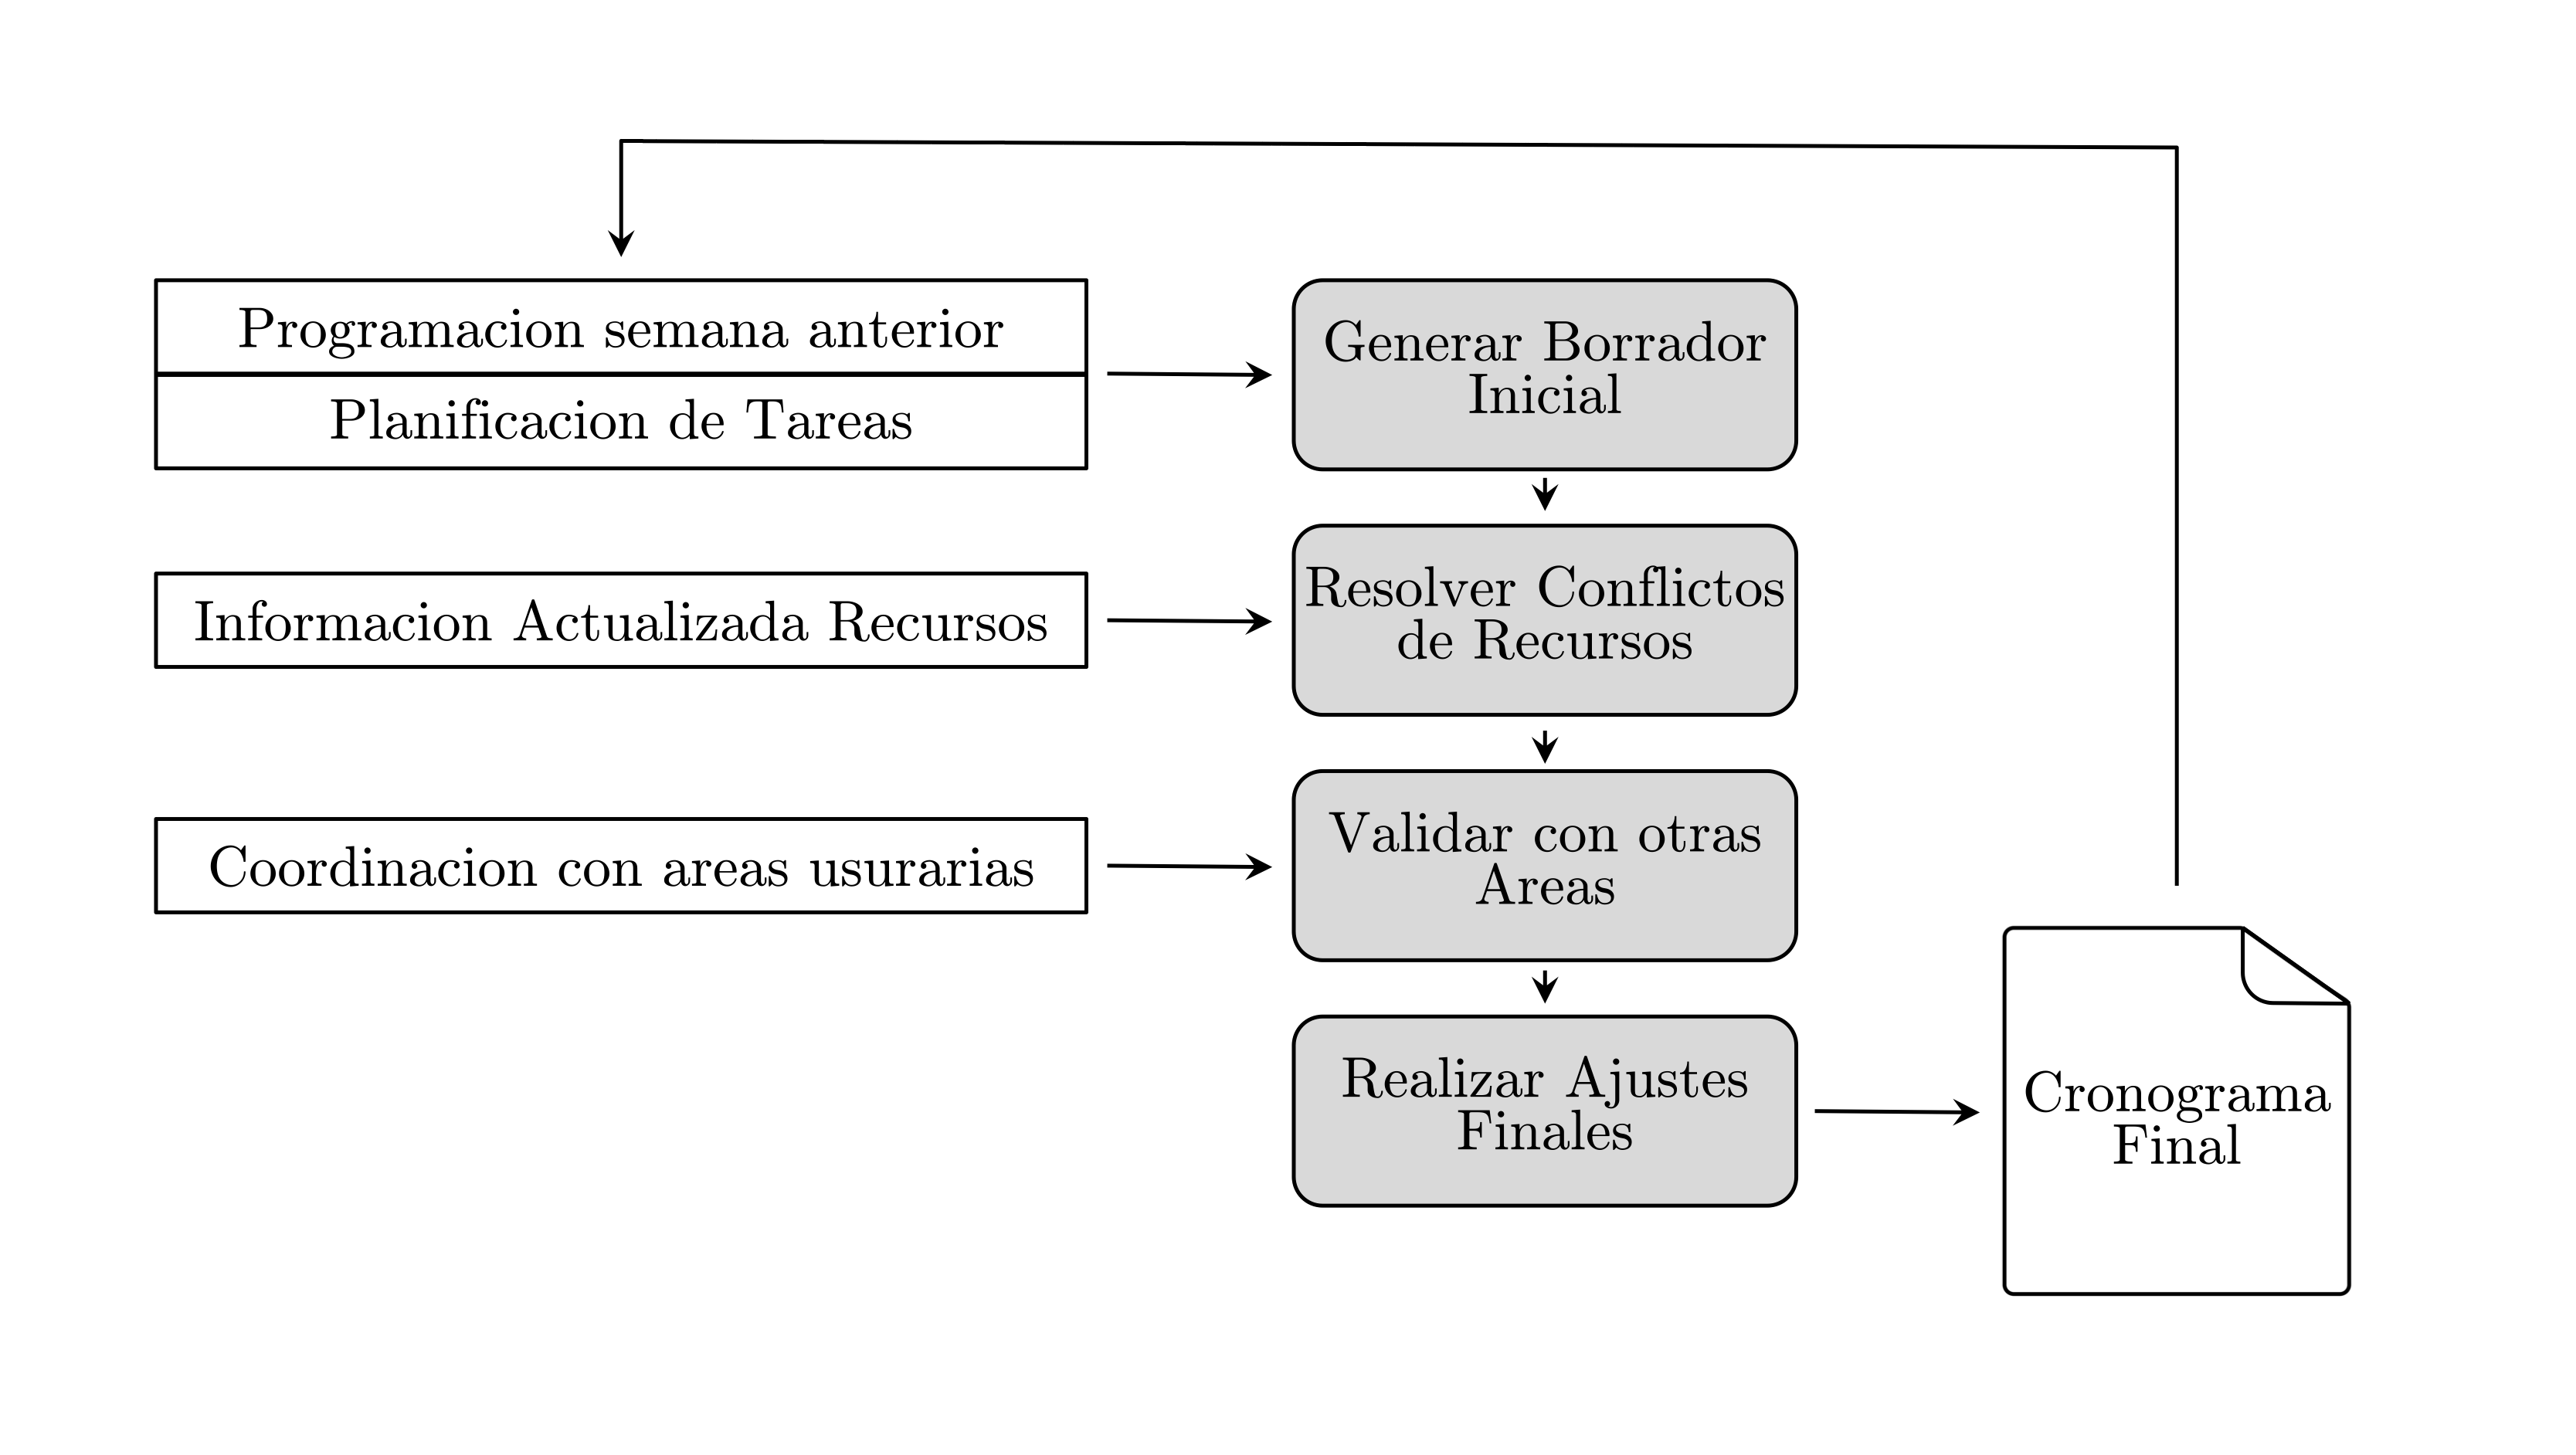
\includegraphics[width=0.75\textwidth]{imgs/process_flowchart.png}}
    \caption{Ciclo Semanal de Programación de Actividades.}
    \label{fig:flowchart}
\end{figure}


El cronograma resultante detalla las tareas a realizar, la fecha y hora de inicio, la duración y los recursos necesarios. Este proceso también considera tareas en función de su criticidad, priorizando aquellas que tienen mayor impacto en la continuidad operativa.

\subsubsection{Ciclo Semanal de Programación}

El proceso de programación en el área de mantenimiento se organiza en un ciclo semanal, cuyo objetivo es garantizar que el cronograma sea factible, actualizado y aprobado por las áreas involucradas, alineándose con los requerimientos del negocio y la disponibilidad de recursos.

Cada miércoles, el equipo de programación toma como base el cronograma generado en el ciclo de la semana anterior, que ya contiene actividades programadas para la semana actual. Este cronograma inicial es revisado y ajustado, incorporando nuevas tareas provenientes del proceso de planificación y actualizando la disponibilidad de recursos. Con esta información, se genera el borrador del cronograma que abarca las próximas tres semanas.

El borrador se valida en conjunto con otras áreas para resolver conflictos de recursos y ajustar prioridades. Finalmente, cada viernes se emite el cronograma oficial, que servirá de base para el próximo ciclo. Este enfoque iterativo asegura que la programación sea dinámica y adaptable, optimizando la continuidad operativa. En la \textbf{Figura \ref{fig:flowchart}} se muestra un diagrama de flujo que resume el ciclo semanal de programación de actividades.


\subsection{Diagnóstico del proceso actual}

Como parte del levantamiento de información para comprender el estado actual del proceso de programación de tareas de mantenimiento, se realizó una encuesta dirigida al personal de programación de la empresa colaboradora. Los resultados permiten identificar aspectos críticos y validar la necesidad de herramientas automatizadas que optimicen la generación de cronogramas. Para ver el detalle de los resultados de la encuesta se puede consultar el \textbf{Anexo \ref{anexo:encuesta}}.

A continuación, se presentan los principales hallazgos y conclusiones derivados del diagnóstico del proceso actual:

\begin{itemize}
    \item \textbf{Alta dedicación horaria}: 64\% de los encuestados invierte más de la mitad de su jornada semanal en generación del cronograma de actividades.
    \item \textbf{La creación del borrador inicial} es la fase más intensiva en tiempo, superando otras actividades como resolver conflictos o validar con otras áreas (Ver \textbf{Figura \ref{fig:pie_chart}}).
    \item \textbf{La no disponibilidad de materiales y repuestos} durante la ejecución de las mantenciones es el error más recurrente.
    \item \textbf{Entorno altamente dinámico}: El 90\% de los encuestados enfrenta cambios de último minuto al menos una vez por semana.
    \item \textbf{Problemas de coordinación con otras áreas} y \textbf{falta de colaboración} son barreras adicionales que dificultan la programación eficiente.
\end{itemize}

Los resultados refuerzan la hipótesis de que el proceso de programación podría beneficiarse significativamente de herramientas que automatizan partes clave del flujo de trabajo. En particular, una solución que automatice la creación del borrador inicial del cronograma y que permita incorporar cambios de último minuto sería de gran utilidad para el equipo de programación.


\begin{figure}[htbp]
    \centering
    \frame{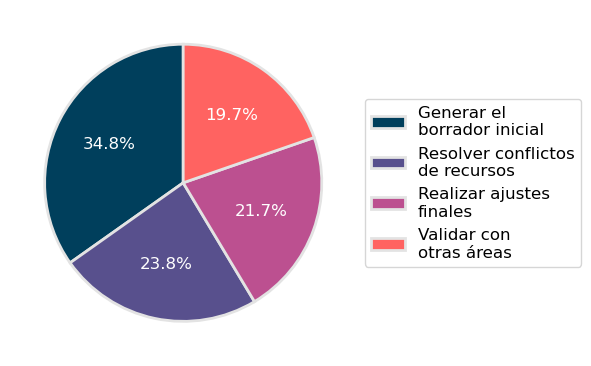
\includegraphics[scale=0.6]{imgs/pie_chart.png}}
    \captionsetup{justification=centering} % Para centrar el texto de la leyenda
    \caption{Distribución del tiempo de programación \\ \textbf{Fuente}: Elaboración propia en base a encuesta (Anexo \ref{anexo:encuesta})}
    \label{fig:pie_chart}
  \end{figure}

\section{Definiciones teóricas}
En este apartado se presentan las definiciones y conceptos teóricos fundamentales para comprender el enfoque del proyecto. Se abordan el \textit{RCPSP} y los algoritmos \textit{CP}. Estos conceptos son esenciales para entender las metodologías utilizadas en nuestra solución para la programación de actividades de mantenimiento.

\subsection{Problema de Programación de Proyectos con Restricciones de Recursos (\textit{RCPSP})}
El \textit{RCPSP} es un problema clásico en el campo de la investigación operativa y la gestión de proyectos. Cabe dentro de los \textit{Constraint Satisfaction Problems} (CSP) y más especificamente dentro de los \textit{Constraint Optimization Problems} (COP).

Consiste en programar un conjunto de actividades interrelacionadas, considerando restricciones tanto de precedencia entre tareas como de disponibilidad limitada de recursos. El objetivo principal es determinar el calendario óptimo que minimice la duración total del proyecto (\textit{makespan}) o que optimice otro criterio relevante, como costos o utilización de recursos\cite{artigues2008resource}.
    

Las principales características del \textit{RCPSP} incluyen:
\begin{itemize}
  \item \textbf{Restricciones de precedencia}: Algunas actividades no pueden comenzar hasta que otras hayan finalizado
  \item \textbf{Recursos limitados}: Los recursos necesarios para realizar las actividades (como mano de obra, equipos o materiales) tienen una disponibilidad limitada en cada periodo de tiempo.
  \item \textbf{Objetivo de optimización}: Generalmente, se busca minimizar el tiempo total del proyecto, aunque pueden considerarse otros objetivos como minimizar costos o equilibrar la carga de recursos.
\end{itemize}

En la \textbf{Figura \ref{fig:rcpsp}} se muestra un ejemplo de un \textit{RCPSP} con 2 recursos y 10 tareas. En él se muestra que el Recurso A tiene una capacidad de 7 unidades mientras que el Recurso B tiene una capacidad de 4 unidades. Dadas los requerimientos de recursos de cada tarea y las capacidades de cada recurso, en la figura se muestra una solución que logra un \textit{makespan} de 12 unidades de tiempo.

\begin{figure}[htbp]
    \centering
    \frame{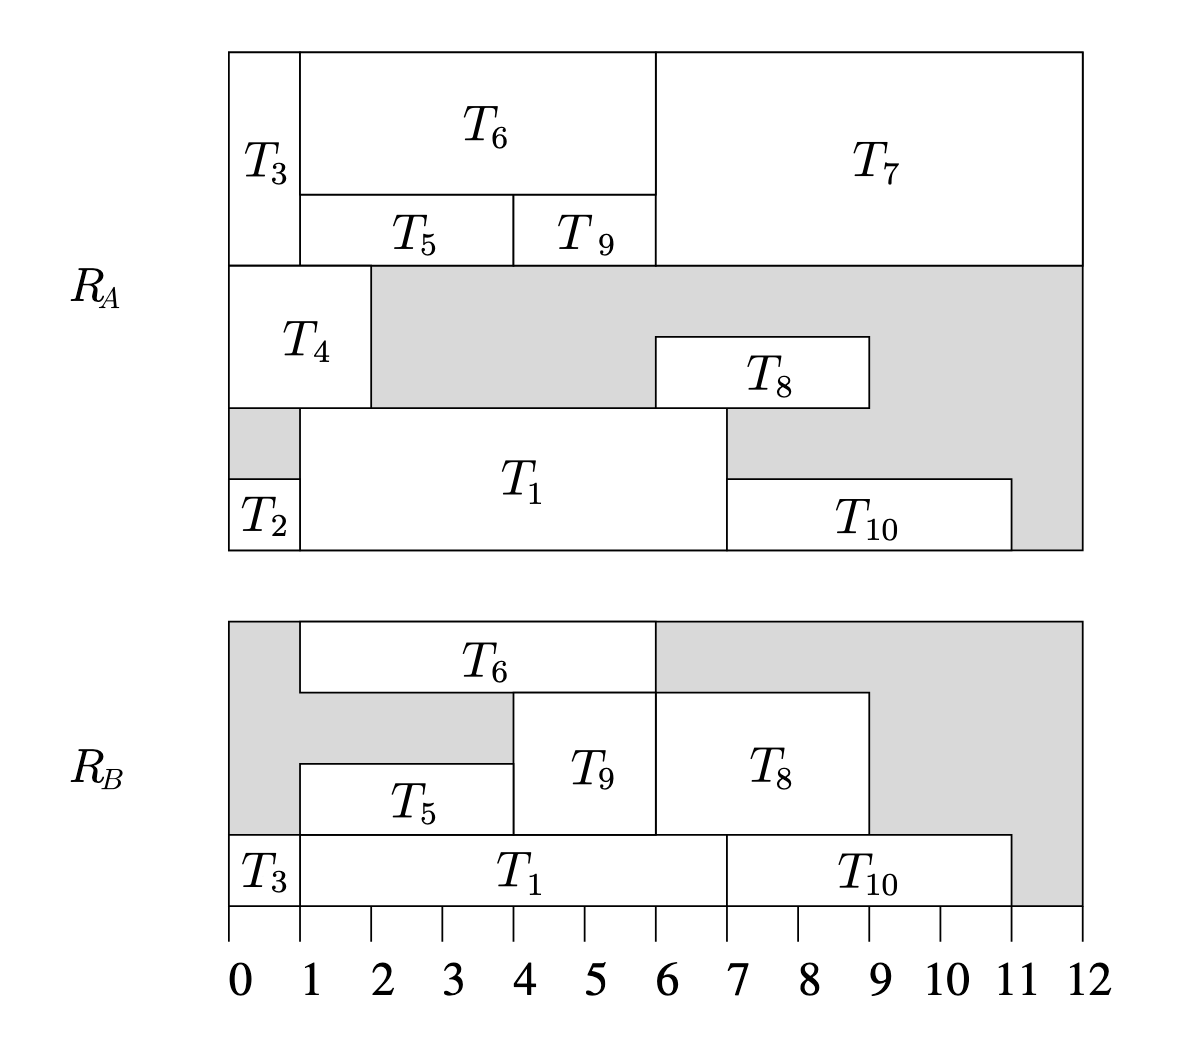
\includegraphics[width=0.5\textwidth]{imgs/rcpsp.png}}
    \caption{Ejemplo de un \textit{RCPSP} con 2 recursos y 10 tareas.}
    \label{fig:rcpsp}
\end{figure}
    

El \textit{RCPSP} es reconocido como un problema NP-Hard, lo que significa que no se dispone de un algoritmo que pueda resolver todas sus instancias en tiempo polinomial, dada la complejidad inherente al crecimiento exponencial del espacio de soluciones conforme aumenta el número de tareas y recursos involucrados.

Si bien para instancias reducidas pueden aplicarse métodos exactos, la escalabilidad del problema suele requerir el uso de enfoques alternativos. En este sentido, \textit{CP} resulta una herramienta especialmente eficaz, ya que permite modelar y resolver el \textit{RCPSP} de forma declarativa, aprovechando técnicas de propagación de restricciones y búsqueda guiada.



\subsection{Algoritmos de Programación por Restricciones (\textit{CP})}

\textit{CP} es una técnica ampliamente utilizada para resolver problemas combinatorios complejos, como los problemas de programación y planificación de actividades. En el contexto de este trabajo, \textit{CP} es fundamental para abordar el \textit{RCPSP}, proporcionando un marco eficaz para modelar y resolver problemas que incluyen restricciones de tiempo y recursos.

Un problema de satisfacción de restricciones (\textit{Constraint Satisfaction Problem}, \textit{CSP}) se define como un conjunto de variables  $V$ , cada una asociada a un dominio de valores posibles  $D$ , y un conjunto de restricciones  $R$  que especifican las combinaciones válidas de valores entre las variables. La solución a un CSP es una asignación de valores a las variables que satisface todas las restricciones. Cuando se incorpora una función objetivo  $O$  para optimizar, el problema se denomina \textit{Constraint Optimization Problem} (\textit{COP})\cite{rossi2006}. En la \textbf{Figura \ref{fig:constraint_programming}} se muestra un esquema general de \textit{COP}.

\begin{figure}[htbp]
\centering
\frame{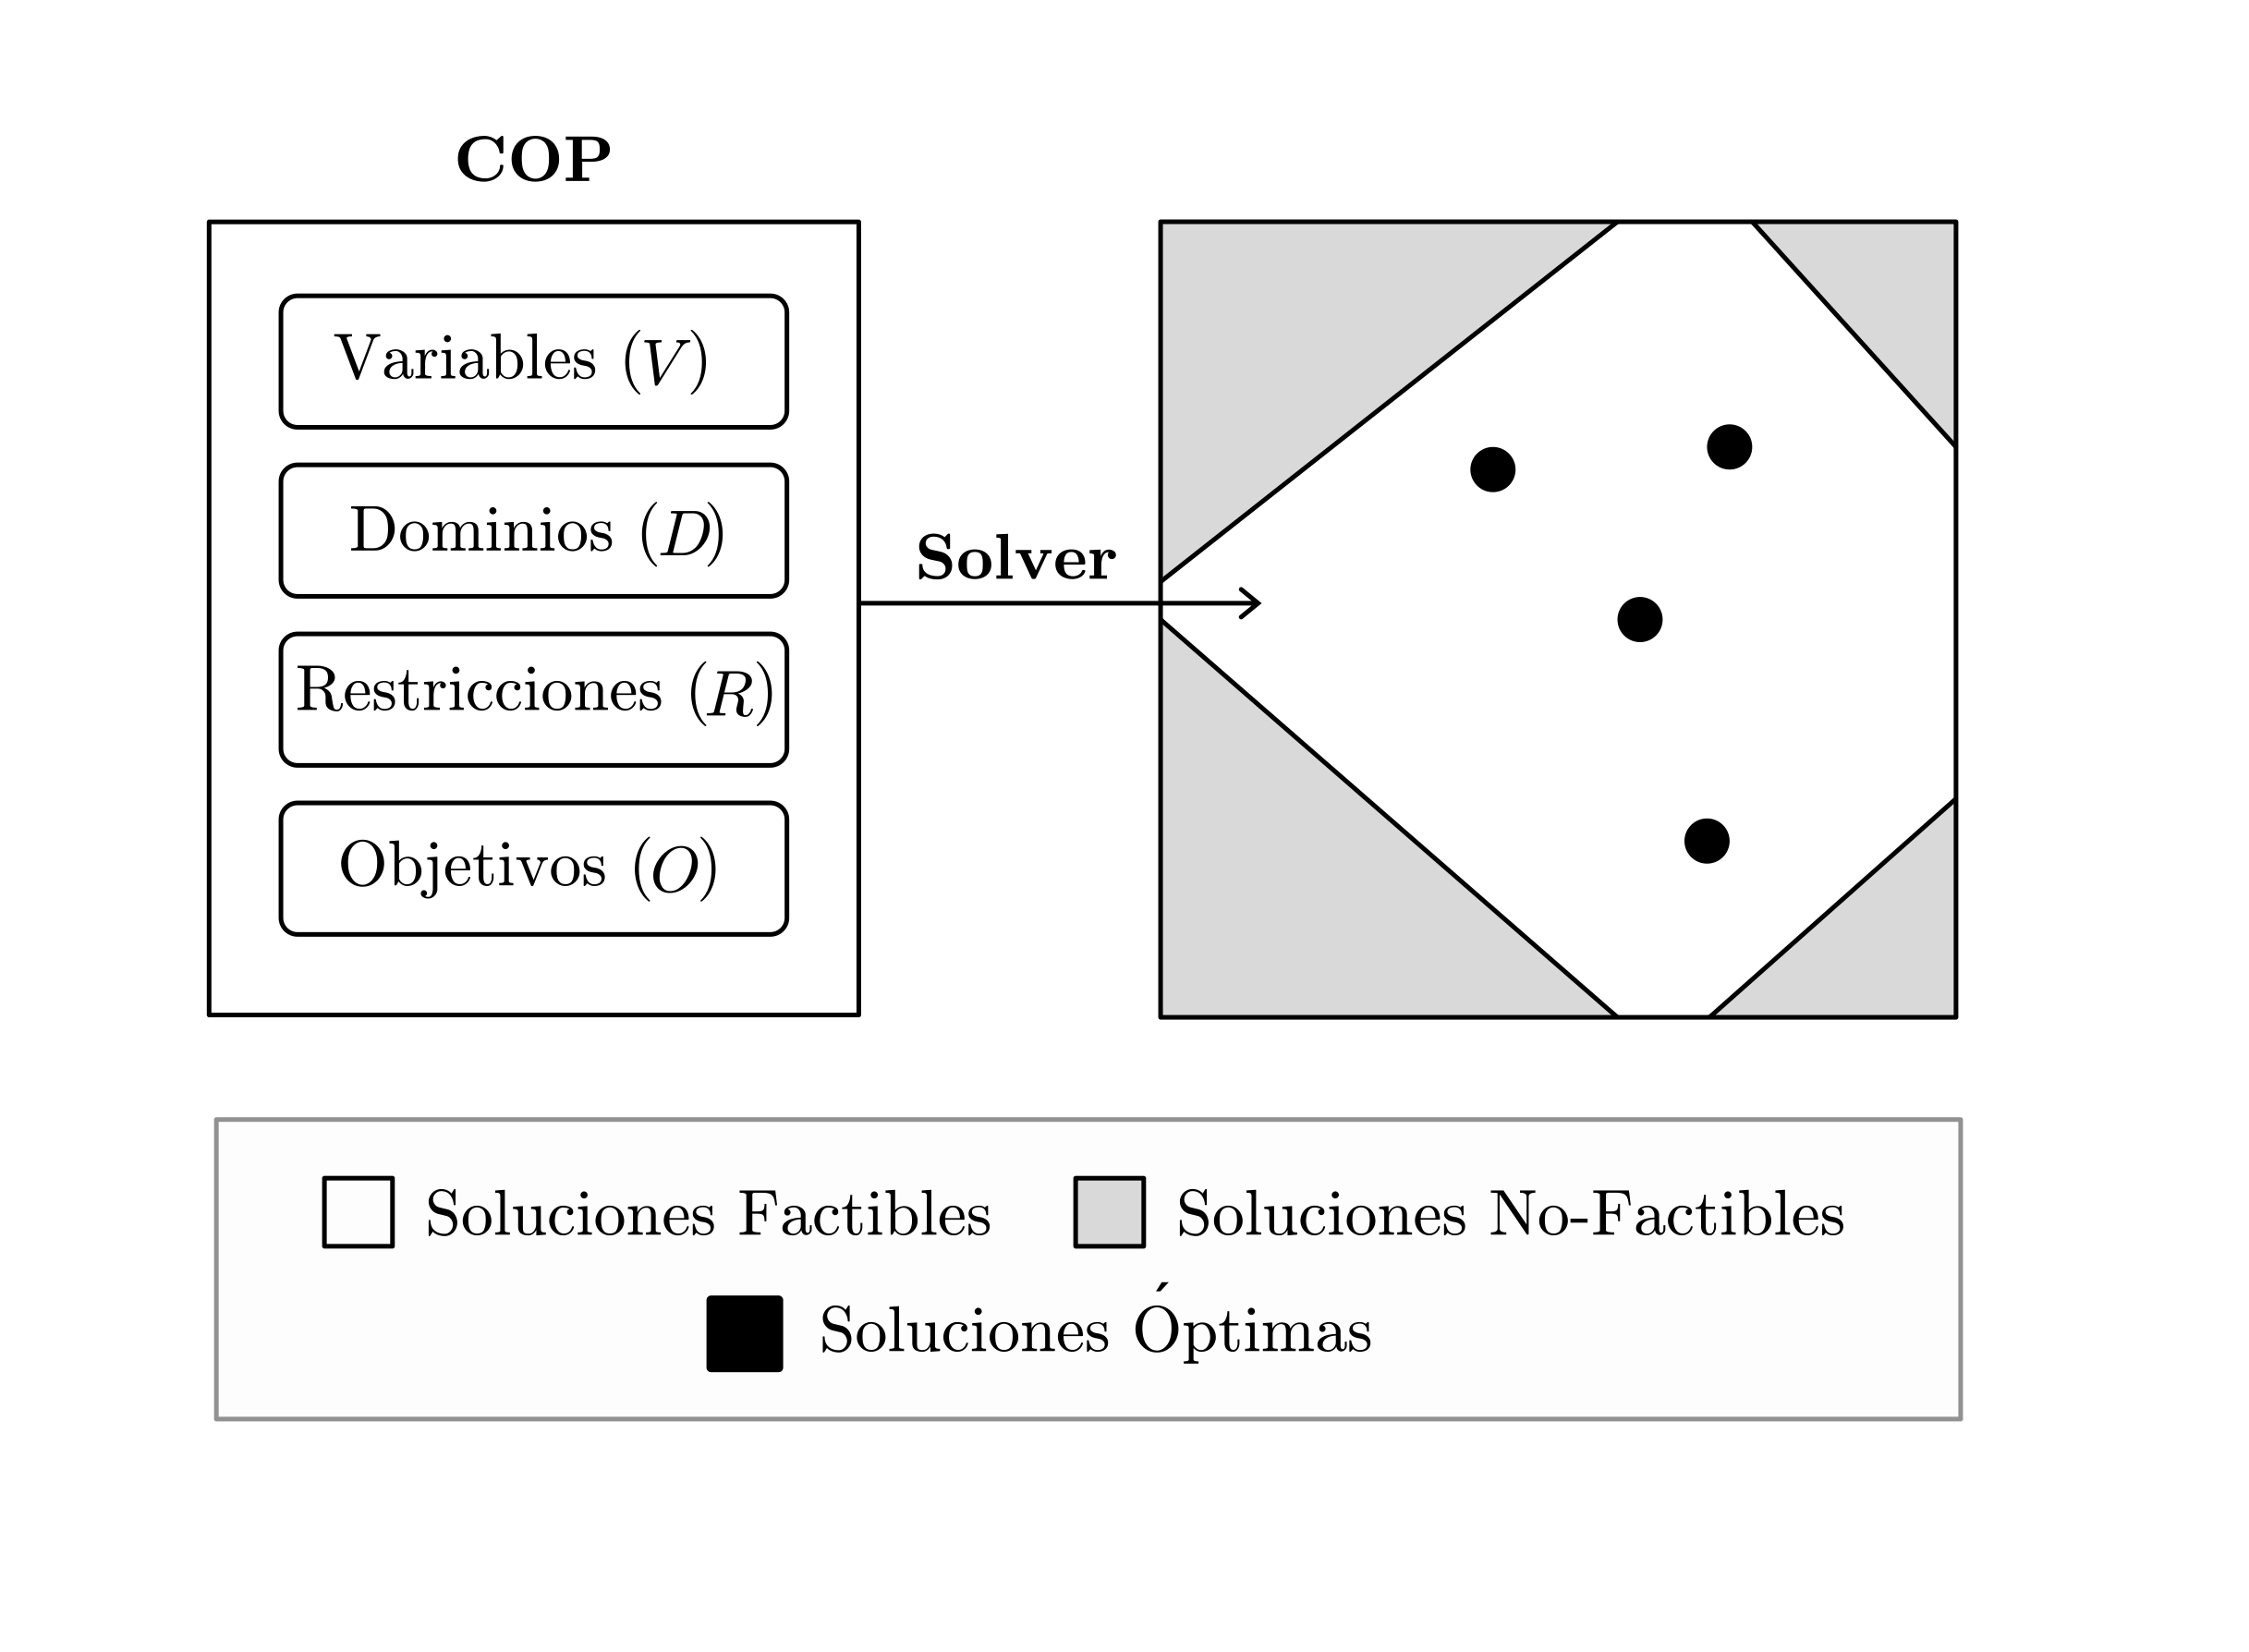
\includegraphics[width=0.75\textwidth]{imgs/constraint_programming.png}}
\caption{Esquema de Programación con Restricciones.}
\label{fig:constraint_programming}
\end{figure}

En el contexto del \textit{RCPSP}, \textit{CP} permite representar las actividades mediante variables de inicio, duración y fin. Las restricciones temporales, como las de precedencia, aseguran que el orden de ejecución sea respetado, mientras que las restricciones de recursos garantizan que no se exceda la capacidad disponible en ningún momento. Además, las ventanas temporales asociadas a cada tarea reflejan los plazos operativos.

La función objetivo de este tipo de problemas puede variar, siendo común la minimización del \textit{makespan}. \textit{CP} permite, además, modelar estos problemas de manera declarativa, separando la especificación del modelo de los algoritmos utilizados para resolverlo. Esto facilita la extensión y modificación de los modelos, adaptándolos a las necesidades específicas sin comprometer la eficacia de los métodos de solución.


% \subsection{Algoritmos de Programación por Restricciones}
% Los algoritmos de Programación por Restricciones son técnicas avanzadas de optimización que se utilizan para resolver problemas combinatorios complejos, como el Problema de Programación de Proyectos con Restricciones de Recursos (RCPSP). Estos algoritmos son especialmente efectivos debido a su capacidad para manejar de manera eficiente restricciones lógicas, aritméticas y de recursos.

% La Programación por Restricciones es un paradigma en el que se definen variables, dominios y restricciones. Las variables representan los elementos desconocidos del problema, los dominios especifican los posibles valores que pueden tomar, y las restricciones limitan las combinaciones de valores que las variables pueden asumir simultáneamente. El objetivo es encontrar asignaciones de valores a las variables que satisfagan todas las restricciones impuestas. Este enfoque es especialmente útil cuando las restricciones son numerosas y complejas, permitiendo modelar problemas de manera flexible y detallada.

% En el contexto del RCPSP, los algoritmos de Programación por Restricciones ofrecen un marco poderoso para modelar y resolver el problema de manera eficiente. Se definen variables de inicio y fin para cada tarea, así como variables de intervalo que combinan inicio, duración y fin, facilitando el manejo de restricciones temporales y de recursos. Las restricciones de precedencia se establecen para asegurar que una tarea no pueda comenzar hasta que sus tareas precedentes hayan finalizado, lo cual se expresa mediante relaciones de desigualdad entre las variables de fin e inicio de las tareas involucradas.

% Las restricciones de recursos se manejan mediante la restricción cumulativa, que garantiza que, en cualquier momento, la suma de los recursos consumidos por las tareas en ejecución no exceda la capacidad disponible. Esto es crucial en problemas donde los recursos son limitados y deben ser compartidos entre múltiples tareas. Además, se consideran las ventanas de tiempo para las tareas, imponiendo límites en las variables de inicio y fin según las fechas de inicio más tempranas y las fechas límite, lo que refleja la disponibilidad y los plazos específicos de cada tarea.

% La función objetivo en estos problemas suele ser minimizar el makespan, es decir, el tiempo total del proyecto. Los algoritmos de Programación por Restricciones permiten integrar esta función objetivo en el modelo, buscando no solo soluciones factibles que satisfagan todas las restricciones, sino también optimizar este criterio para mejorar la eficiencia global del proyecto.

% Una de las ventajas clave de los algoritmos de Programación por Restricciones es su eficiencia en el manejo de restricciones complejas, permitiendo resolver problemas NP-Hard como el RCPSP en tiempos razonables. Su flexibilidad permite incorporar fácilmente nuevas restricciones o modificar las existentes sin reestructurar todo el modelo, lo que es especialmente útil en entornos dinámicos donde las condiciones pueden cambiar. Además, son capaces de encontrar soluciones de alta calidad, óptimas o cercanas al óptimo, lo cual es esencial en contextos industriales donde la optimización de recursos y tiempos es crítica.


\section{Aplicación de los conceptos teóricos al problema}

En esta sección se describe cómo los conceptos teóricos del \textit{RCPSP} y \textit{CP} se aplican al diseño e implementación de nuestra solución para la programación de tareas. Se detallan los datos necesarios para el \textit{input}, las consideraciones al programar, y la generalización del problema como un modelo matemático.

\subsection{Datos necesarios para el proceso de programación}  

El proceso de programación requiere como \textit{input} el resultado del proceso de planificación, que define los parámetros esenciales para cada tarea. Esta información incluye una descripción general de la tarea, indicando a qué orden de trabajo corresponde, además de datos sobre la ventana de fechas en la que debe ejecutarse. También se especifica la duración de la tarea, su nivel de criticidad y los recursos necesarios para ejecutarla, como cuadrillas y equipos. El detalle de una tarea estándar con toda esta información se puede consultar en el \textbf{Cuadro \ref{table:task}}.  

Además de la información proveniente del proceso de planificación, es necesario extraer datos adicionales desde el sistema \textit{ERP} de la empresa. Esto incluye los turnos de las cuadrillas, y la disponibilidad de los equipos auxiliares. Asimismo, es importante también incorporar en el análisis la disponibilidad de materiales y repuestos, sin embargo, dado que estos datos no se encuentran sistematizados en el \textit{ERP}, no se considerarán en este trabajo.


\begin{table}[htbp]
    \centering
    \captionsetup{justification=centering}
    \vspace{0.5cm}
    \begin{tabular}{p{6cm} p{8cm}}
        \toprule
        \textbf{Atributo} & \textbf{Descripción} \\
        \midrule
        \textbf{ID Orden de Trabajo} & 4000001 \\
        \textbf{ID Tarea} & 001 \\
        \textbf{Descripción OT} & Cambio de suspensión trasera lado izquierdo \\
        \textbf{Descripción Tarea} & Retiro de suspensión trasera \\
        \textbf{Fecha Inicio Extrema} & 2024-11-29 \\
        \textbf{Fecha Requerida} & 2024-12-30 \\
        \textbf{Cuadrilla} & BM001 \\
        \textbf{Equipo Auxiliar} & Alza Hombres Telescópico \\
        \textbf{Duración (horas)} & 6 \\
        \textbf{Criticidad} & 2 \\
        \textbf{Cantidad de Trabajadores} & 4 \\
        \bottomrule
    \end{tabular}
    \caption{Ejemplo de Tarea y sus atributos.}
    \label{table:task}
\end{table}


\subsection{Consideraciones al Programar}
El proceso de programación de actividades de mantenimiento implica que el programador tome las órdenes de trabajo pendientes y agende cada una de las tareas considerando su compatibilidad con los horarios y restricciones de otras actividades y de los recursos. Se deben tener en cuenta las siguientes consideraciones:

\begin{itemize}
    \item Cada \textbf{tarea} viene acompañada de información esencial, asignada en el proceso de planificación. Dentro de esta información tenemos la fecha de inicio extrema, la fecha requerida, la duracion, los recursos requeridos y la criticidad.
    \item Dentro de cada \textbf{orden de trabajo}, las tareas tienen restricciones de precedencia, lo que implica que una tarea no puede comenzar hasta que la tarea anterior haya finalizado.
    
    \item Cada \textbf{cuadrilla} tiene su propio esquema de turnos, lo que implica que hay ventanas de tiempo en las cuales estos recursos no están diponibles.
    
    \item Cada \textbf{cuadrilla} tiene una capacidad determinada, que corresponde al número de trabajadores disponibles, lo que influye en la cantidad de tareas que pueden realizarse simultáneamente. Por ejemplo, si una cuadrilla tiene una capacidad de 10 trabajadores, podrá ejecutar 5 tareas que requieran 2 trabajadores cada una de manera simultánea.
    \item Los \textbf{equipos auxiliares} son unitarios, por lo tanto no pueden asignarse a más de una tarea simultaneamente.
    \item Generalmente los programadores se basan en \textbf{cronogramas generados en semanas anteriores}, sobre el cual hacen ajustes o incorporan las tareas nuevas que van ingresando.
    \item Si se programa una tarea de una \textbf{Orden de Trabajo}, todas las tareas de esa OT deben ser programadas.

\end{itemize}


\subsection{Generalización del Problema como \textit{RCPSP}}

Vamos a modelar el problema de programación de tareas de la empresa colaboradora como un \textit{RCPSP}. El objetivo es asignar tiempos de inicio a las tareas, minimizando el \textit{makespan} y minimizando la cantidad de tareas no programadas. Se consideran también las restricciones de capacidad de los recursos, las ventanas de tiempo, los intervalos prohibidos y las posibles relaciones de precedencia entre tareas.

A continuación, se presenta una descripción general del modelo de programación de tareas con recursos limitados que servirá como base para la implementación de la solución.

\subsubsection{Parámetros del Modelo}

Tenemos los siguientes elementos:

\textbf{Tareas}: Un conjunto \( T = \{T_0, T_1, \dots, T_n\} \), donde cada tarea \( T_i \) tiene:
  \begin{itemize}
    \item Una duración \( C(T_i) \in \mathbb{N} \).
    \item Un conjunto de recursos requeridos \( D(T_i) \subseteq R \).
    \item Una cantidad del recurso requerido \( q_i \in \mathbb{N} \).
    \item Una criticidad \( \text{Impact}_i \in \mathbb{N} \), donde un valor más bajo indica mayor prioridad.
    \item Una ventana de tiempo \( W(T_i) = [\text{early}_i, \text{late}_i] \), que indica el tiempo más temprano y más tardío en el que puede comenzar la tarea.
  \end{itemize}

\textbf{Recursos}: Un conjunto \( R = \{R_0, R_1, \dots, R_m\} \), donde cada recurso \( R_j \) tiene:
  \begin{itemize}
    \item Una capacidad \( P(R_j) \in \mathbb{N} \).
    \item Un conjunto de intervalos prohibidos \( I(R_j) = \{[a_1, b_1), [a_2, b_2), \dots\} \), durante los cuales el recurso no está disponible.
  \end{itemize}

\textbf{Grupos de tareas}: Un conjunto \( G = \{G_0, G_1, \dots\} \), donde cada grupo \( G_k \subseteq T \) tiene restricciones de precedencia entre las tareas que lo componen.

\vspace{0.5cm}

\begin{tcolorbox}[colback=gray!5!white, colframe=gray!75!black, title={Parámetros del modelo}]
    \begin{itemize}
        \item \( T = \{T_0, T_1, \dots, T_n\} \): conjunto de \textbf{tareas}.
        \item \( R = \{R_0, R_1, \dots, R_m\} \): conjunto de \textbf{recursos}.
        \item \( C(T_i) \in \mathbb{N} \): \textbf{duración} de la tarea \( T_i \).
        \item \( D(T_i) \subseteq R \): \textbf{recursos requeridos} por la tarea \( T_i \).
        \item \( q_i \in \mathbb{N} \): \textbf{cantidad} de recurso que requiere la tarea \( T_i \).
        \item \( \text{Impact}_i \in \mathbb{N} \): \textbf{criticidad} de la tarea \( T_i \) (prioridad inversa).
        \item \( W(T_i) = [\text{early}_i, \text{late}_i] \): \textbf{ventana de tiempo} para la tarea \( T_i \).
        \item \( P(R_j) \in \mathbb{N} \): \textbf{capacidad} del recurso \( R_j \).
        \item \( I(R_j) = \{[a_k, b_k)\} \): \textbf{intervalos prohibidos} del recurso \( R_j \).
        \item \( G = \{G_0, G_1, \dots\} \): conjunto de \textbf{grupos de tareas} con restricciones de precedencia.
    \end{itemize}
\end{tcolorbox}

\vspace{0.5cm}

\subsubsection{Variables de decisión}

Para modelar el problema, introducimos las siguientes variables de decisión:

\begin{itemize}
    \item \( x_i \in \{0, 1\} \): Indica si la tarea \( T_i \) es \textbf{programada} (\( x_i = 1 \)) o no (\( x_i = 0 \)).
    \item \( S_i \in \mathbb{N} \): Tiempo de \textbf{inicio} de la tarea \( T_i \), sujeto a \( \text{early}_i \leq S_i \leq \text{late}_i - C(T_i) \) si \( x_i = 1 \).
    \item \( E_i = S_i + C(T_i) \): Tiempo de \textbf{finalización} de la tarea \( T_i \).
    \item \( \text{Intervalo}(T_i) = [S_i, E_i) \): Intervalo de ejecución de la tarea \( T_i \).
    \item \( y_k \in \{0, 1\} \): Indica si el \textbf{grupo de tareas} \( G_k \) es programado (\( y_k = 1 \)) o no (\( y_k = 0 \)).
\end{itemize}

\vspace{0.5cm}

\begin{tcolorbox}[colback=gray!5!white, colframe=gray!75!black, title={Variables de decisión}]
    \begin{itemize}
        \item \( x_i \in \{0, 1\} \): Variable binaria que indica si la tarea \( T_i \) es \textbf{programada}.
        \item \( S_i \in \mathbb{N} \): Tiempo de \textbf{inicio} de la tarea \( T_i \).
        \item \( E_i = S_i + C(T_i) \): Tiempo de \textbf{finalización} de la tarea \( T_i \).
        \item \( \text{Intervalo}(T_i) = [S_i, E_i) \): Intervalo de ejecución de la tarea \( T_i \).
        \item \( y_k \in \{0, 1\} \): Variable binaria que indica si el grupo \( G_k \) es \textbf{programado}.
    \end{itemize}
\end{tcolorbox}

\vspace{0.5cm}

\subsubsection{Restricciones}

El modelo considera las siguientes 5 restricciones:

\textbf{a. Ventanas de tiempo}:

Cada tarea debe comenzar y finalizar dentro de su ventana de tiempo permitida si es programada:

\[
x_i = 1 \implies \text{early}_i \leq S_i \leq \text{late}_i - C(T_i)
\]

\textbf{b. Restricciones de capacidad de los recursos}:

Para cada recurso \( R_j \), la suma de las demandas de las tareas que requieren el recurso en cualquier momento no debe exceder su capacidad:

\[
\sum_{\substack{T_i \in T \\ R_j \in D(T_i)}} q_i \cdot \delta_{ij}(t) \leq P(R_j), \quad \forall t \in \text{Horizonte}
\]

Donde \( \delta_{ij}(t) = 1 \) si \( t \in [S_i, E_i) \) y \( x_i = 1 \); en caso contrario, \( \delta_{ij}(t) = 0 \).

\textbf{c. Intervalos prohibidos de los recursos}:

Las tareas no pueden ser programadas durante los intervalos prohibidos de los recursos que requieren:

\[
x_i = 1 \implies \forall R_j \in D(T_i), \forall [a_k, b_k) \in I(R_j): \quad [S_i, E_i) \cap [a_k, b_k) = \emptyset
\]

\textbf{d. Restricciones de precedencia en grupos de tareas}:

Para cada grupo \( G_k \), si el grupo es programado, las tareas deben seguir una secuencia específica:

\[
y_k = 1 \implies \forall T_i, T_{i+1} \in G_k: S_{i+1} \geq E_i
\]

Además, las tareas dentro de un grupo se programan juntas o no se programan:

\[
\forall T_i \in G_k: x_i = y_k
\]

\textbf{e. Consistencia de variables}:

Si una tarea no es programada, sus variables de tiempo no tienen relevancia y pueden ser fijadas a cero para simplificar el modelo:

\[
x_i = 0 \implies S_i = 0, \quad E_i = 0
\]

\vspace{0.5cm}

\subsubsection{Objetivo}

El objetivo es minimizar una combinación del \textit{makespan} global y la penalización asociada a no programar tareas de mayor prioridad. Para esto, se define una función de peso para cada tarea basada en su criticidad:

\[
w_i = (\text{Impact}_{\text{max}} + 1 - \text{Impact}_i)^3
\]

Donde \( \text{Impact}_{\text{max}} \) es el valor máximo de criticidad entre todas las tareas. En este caso \( \text{Impact}_{\text{max}} = 3 \)

La función objetivo es:

\[
\min Z = \alpha \cdot \text{makespan} + \beta \cdot \sum_{i=0}^{n} w_i \cdot (1 - x_i)
\]

Donde:

\begin{itemize}
    \item \( \alpha \): Peso asociado al \textit{makespan} global.
    \item \( \beta \): Peso asociado a la penalización por no programar tareas según su criticidad.
\end{itemize}

Este enfoque busca una solución que equilibre la minimización del \textit{makespan} global y la priorización de tareas críticas según su criticidad.


\subsection{Detalle de Función Objetivo}

Dado que en la práctica puede surgir la posibilidad de que ciertas tareas no puedan ser programadas debido a restricciones como la indisponibilidad de recursos, ventanas de tiempo incompatibles o conflictos en los intervalos prohibidos; es crucial considerar un mecanismo que penalice esta situación pero que la permita, de otro modo cada vez que hayan este tipo de incompatibilidades, el modelo no podrá encontrar una solución factible. 

Por ello, la función objetivo incluye un componente que penaliza la no-programación de tareas. Esto convierte en factibles aquellas soluciones que no logran programar todas las tareas, pero minimiza esta situación tanto como sea posible.

Además, se incluye un componente que penaliza el \textit{makespan}. Este enfoque asegura que el modelo busque simultáneamente programar tantas tareas como sea posible y minimizar el tiempo total requerido para su ejecución.

La función objetivo combina estos dos componentes mediante parámetros de ponderación \( \alpha \) y \( \beta \), que permiten ajustar la importancia relativa de cada criterio en la optimización:

\[
\min Z = \alpha \cdot \text{makespan} + \beta \cdot \sum_{i=0}^{n} w_i \cdot (1 - x_i)
\]

Donde:

\begin{enumerate}
    \item \textbf{Componente del \textit{Makespan} (\( \alpha \cdot \text{makespan} \))}: Busca reducir la extensión global del horizonte temporal necesario para completar todas las tareas programadas, incentivando la eficiencia en el uso de recursos y tiempo.

    \item \textbf{Componente de Penalización por Tareas no Programadas (\( \beta \cdot \sum_{i=0}^{n} w_i \cdot (1 - x_i) \))}: Penaliza la no-programación de tareas, asignando un peso mayor a aquellas con una mayor criticidad. Aquí, \( w_i \) es el peso asociado a la tarea \( T_i \), definido como:
    \[
    w_i = (\text{Impact}_{\text{max}} + 1 - \text{Impact}_i)^3
    \]
    Este peso aumenta de manera cúbica con la criticidad (bajo valor de \( \text{Impact}_i \)) de la tarea, priorizando explícitamente las tareas más importantes.
\end{enumerate}

El uso de \( \alpha \) y \( \beta \) permite al modelo adaptarse a diferentes prioridades operativas. Por ejemplo:

\begin{itemize}
    \item Si \( \alpha \) es significativamente mayor que \( \beta \), el modelo favorecerá soluciones con makespan reducido, aun si algunas tareas críticas no se programan.
    \item Si \( \beta \) domina sobre \( \alpha \), el enfoque se orientará a maximizar la programación de tareas críticas, incluso si eso resulta en un makespan mayor.
\end{itemize}

De esta manera, la función objetivo ofrece un balance flexible que puede ser ajustado según las necesidades específicas del problema, garantizando una solución óptima que considere tanto la completitud de las tareas como la eficiencia global.


%%%%%%%%%%%%%%%%%%%

\section{Diseño de la Solución}

El flujo de trabajo de la solución se ha organizado en cuatro etapas secuenciales, cada una diseñada para estructurar y procesar la información de programación de manera eficiente (Ver \textbf{Figura \ref{fig:solution}}). Estas etapas abarcan desde la ingesta y preparación de datos hasta la generación del cronograma optimizado, en distintos formato. A continuación, se describen las cuatro partes que componen el flujo de trabajo:

\begin{enumerate}
    \item \textbf{Pre-Procesamiento}: Se toman los datos de las tareas desde distintas fuentes (\textit{ERP}, \textit{Microsoft Project}, u otros formatos) y se estandarizan, asegurando que los campos relevantes estén estructurados de manera uniforme.

    \item \textbf{Segmentación en Subconjuntos}: Para mejorar la eficiencia del \textit{solver}, las tareas se agrupan en subconjuntos relacionados. Este proceso identifica conexiones entre tareas mediante relaciones compartidas. La segmentación permite particionar el problema en componentes más manejables, reduciendo la complejidad computacional.

    \item \textbf{\textit{Solver}}: Se utiliza el modelo de \textit{CP} de \textit{OR-Tools} para resolver cada subconjunto de manera independiente, aplicando restricciones y maximizando el cumplimiento de tareas según su prioridad.

    \item \textbf{Post-Procesamiento}: Los resultados obtenidos del \textit{solver} se consolidan y procesan para generar un cronograma unificado. Finalmente, se crean archivos compatibles con herramientas como \textit{Microsoft Project}, facilitando su integración en los flujos de trabajo.
\end{enumerate}

Este flujo de trabajo modular garantiza flexibilidad y adaptabilidad, permitiendo procesar datos de diversas fuentes, optimizar la programación bajo restricciones complejas y generar resultados en formatos útiles para los usuarios finales. A continuación, se describen en detalle cada una de las etapas mencionadas.


\begin{figure}[htbp]
    \centering
    \frame{
\includegraphics[width=.9\textwidth]{imgs/solution.png}}
    \caption{Flujo de Trabajo de la Solución.}
    \label{fig:solution}
\end{figure}

\subsection{Pre-Procesamiento}

La etapa de Pre-Procesamiento constituye el punto de partida del flujo de trabajo, recibiendo y preparando la información procedente de diversas fuentes (como sistemas \textit{ERP}, Microsoft Project u otros formatos externos). Esta fase garantiza que los datos sobre tareas, personal y equipos estén libres de inconsistencias, limpios y normalizados, facilitando así la labor posterior del \textit{solver}.

Las operaciones clave realizadas durante el Pre-Procesamiento incluyen:

\begin{itemize}
    \item \textbf{Corrección de discrepancias}: Se revisan y ajustan datos en caso de encontrar inconsistencias. Por ejemplo, si una tarea presenta una fecha requerida previa a su fecha de inicio extrema, se corrige automáticamente. Asimismo, se unifican los formatos de fechas, duraciones y demás campos relevantes.

    \item \textbf{Cuantización de ventanas horarias}: Las duraciones se expresan en intervalos de 15 minutos para trabajar con unidades enteras en el \textit{solver}. De este modo, una tarea de una hora se representa como 4 unidades, y una tarea de 15 minutos como 1 unidad, optimizando la eficiencia en el modelado de restricciones temporales.
    
    \item \textbf{Restringir Horarios Fijos}: Si el usuario requiere que ciertas tareas se realicen en horarios específicos, se definen estos intervalos para garantizar su cumplimiento. Esto implica modificar la fecha de inicio extrema y la fecha requerida de las tareas correspondientes, además de darle la máxima prioridad.

    \item \textbf{Estandarización en un formato unificado (JSON)}: Tras la limpieza y normalización, la información se organiza en un archivo JSON. Este archivo consolida datos sobre duración de las tareas, recursos requeridos, ventanas temporales y dependencias, garantizando un formato coherente que servirá de base para las etapas posteriores.

\end{itemize}



\subsection{Segmentación en Subconjuntos}

La Segmentación en Subconjuntos tiene como objetivo reducir la complejidad del problema, dividiendo el conjunto global de tareas en grupos más pequeños y manejables. Este proceso se basa en la identificación de dependencias entre tareas, garantizando que aquellas actividades que comparten recursos se mantengan dentro de un mismo subconjunto.

El método para llevar a cabo esta segmentación es el siguiente:

\begin{enumerate}[label=\alph*.]
    \item \textbf{Construcción del grafo}: Se modelan cuadrillas y equipos auxiliares como nodos de un grafo no dirigido, añadiendo aristas entre dos nodos cuando existen tareas que comparten aquellos recursos.
    
    \item \textbf{Identificación de componentes conexos}: A través de algoritmos de componentes conexos, se detectan grupos de nodos interrelacionados. Cada componente conexo representa un subconjunto de tareas que deben mantenerse juntas para preservar la coherencia en el uso de recursos y las dependencias.

    \item \textbf{Formación de subconjuntos}: Cada componente conexo determina un subconjunto de tareas que se tratará de manera independiente en el \textit{solver}. Esto permite abordar el problema en etapas más pequeñas, reduciendo el número de variables y restricciones manejadas de forma simultánea.
\end{enumerate}


\begin{figure}[htbp]
    \centering
    \frame{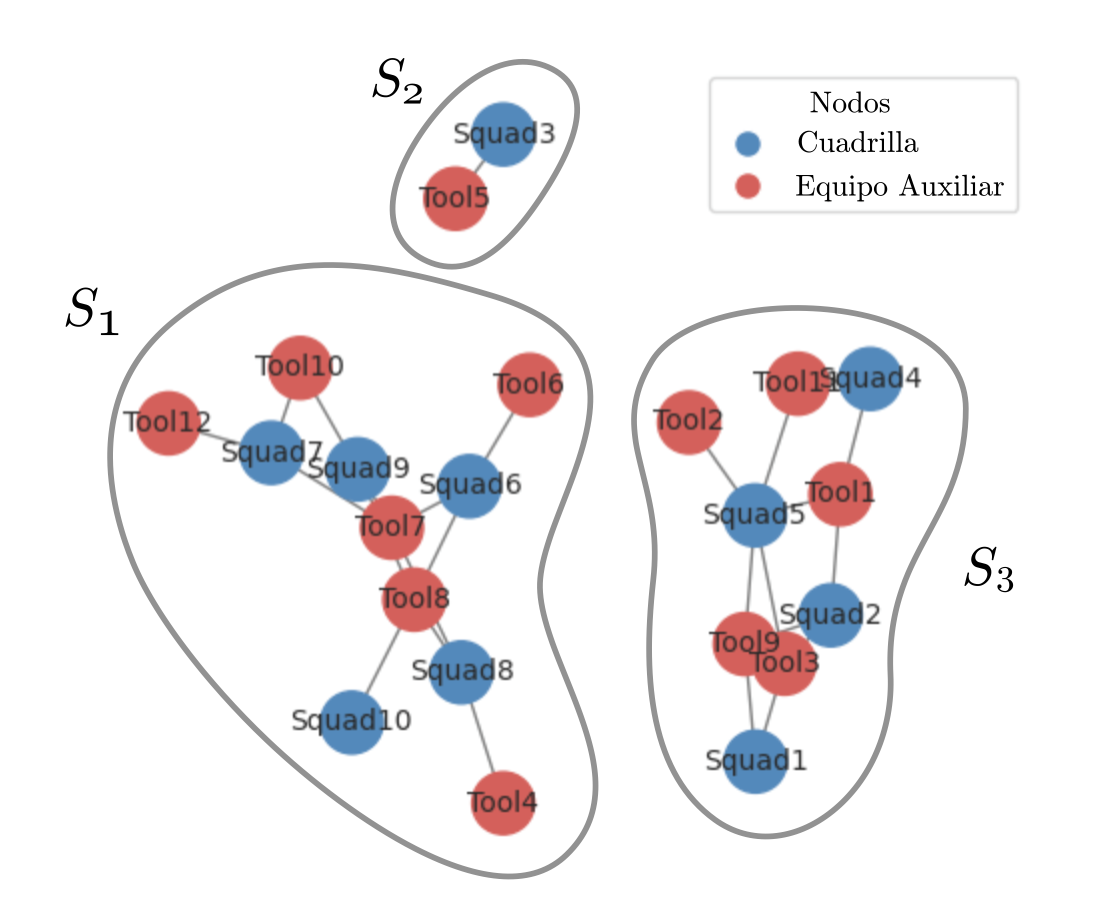
\includegraphics[width=0.5\textwidth]{imgs/segmentacion.png}}
    \caption{Ejemplo de segmentación a través de componentes conexos.}
    \label{fig:segmentacion}
\end{figure}


Gracias a este enfoque, la complejidad computacional disminuye, se mantiene la coherencia en el uso compartido de recursos y es posible resolver cada subconjunto en paralelo, optimizando el uso de recursos computacionales y disminuyendo el tiempo total de cálculo. En la \textbf{Figura \ref{fig:segmentacion}} se muestra un ejemplo de segmentación de tareas en subconjuntos a través de componentes conexos.


\subsection{\textit{Solver}}

A partir de los JSON de cada subconjunto de tareas se construyen los diccionarios que servirán como \textit{input} del \textit{solver}:

\begin{itemize}
    \item \textbf{Diccionario de tareas}: Contiene la duración, recursos y herramientas requeridas por cada tarea, junto con las variables clave del modelo (inicio, fin, entre otros).

    \item \textbf{Diccionario de ventanas de tiempo}: Especifica para cada tarea sus límites temporales, a fin de asegurar el cumplimiento de las restricciones temporales definidas.

    \item \textbf{Diccionario de capacidades de recursos}: Detalla la disponibilidad máxima de cada recurso, garantizando que no se sobrepase su límite durante la programación.

    \item \textbf{Diccionario de agrupaciones de tareas}: Define conjuntos de tareas (OTs) que comparten recursos o secuencias de precedencia, facilitando la coherencia en la programación de actividades relacionadas.

    \item \textbf{Diccionario de intervalos prohibidos}: Registra los periodos en los que ciertos recursos no están disponibles, asegurando que no se asignen tareas en dichos intervalos.

    \item \textbf{Diccionario de horarios preferenciales}: Incluye el horario preferente para ciertas tareas. Se usa cuando se trabaja sobre un cronograma previo y se desea mantener ciertas tareas en los mismos horarios, dentro de lo posible.

\end{itemize}



Luego, para resolver cada uno de los subconjuntos de tareas se utiliza el \textit{solver} de CP de la librería \textit{OR-Tools} de \textit{Python}. Esta herramienta permite modelar problemas complejos de programación con restricciones, aprovechando las estructuras de datos preparadas en la etapa de Pre-Procesamiento.

En el caso en el que se trabaja con un cronograma previo, se incorporan las tareas de este cronograma en el modelo, utilizando el método \verb|add_hint| de \textit{OR-Tools}. Esto permite que el usuario pueda hacer ajustes finos sobre el cronograma anterior, manteniendo las tareas en los horarios preferidos, siempre que sea posible.

Para mejorar el desempeño, se aplican estrategias de paralelización con librerías como \texttt{joblib}, ejecutando la resolución de múltiples subconjuntos de forma simultánea en diferentes hilos o núcleos de procesamiento.


\subsection{Post-Procesamiento}

La fase de Post-Procesamiento consolida los resultados generados por el \textit{solver} y los prepara en formatos finales útiles para su análisis, integración o visualización en herramientas externas.

Partiendo del archivo JSON producido por el \textit{solver} (que indica para cada tarea si fue programada y su hora de inicio), se procesan estos datos junto con la información original, produciendo:

\begin{itemize}
    \item \textbf{Archivos XML para \textit{Microsoft Project}}: Se genera un archivo compatible con \textit{MS Project}, conteniendo horas de inicio, finalización y duraciones, facilitando la incorporación del cronograma en flujos de trabajo existentes.

    \item \textbf{Archivo XLSX para \textit{Microsoft Excel}}: Se produce una carta Gantt en \textit{MS Excel}, organizando las tareas en un cronograma visual y detallando inicio, fin, duración, así como los recursos asignados, permitiendo una int\textit{erp}retación rápida y clara.

    \item \textbf{Integraciones con APIs empresariales}: Si la organización cuenta con sistemas \textit{ERP} u otros entornos de gestión, los resultados pueden integrarse automáticamente mediante APIs, asegurando la continuidad operativa y minimizando el trabajo manual.
\end{itemize}

El Post-Procesamiento garantiza que los resultados generados por el \textit{solver} sean comunicados de forma clara y estén listos para su explotación por usuarios finales, herramientas de gestión o análisis posterior. De este modo, el flujo de trabajo se completa con un producto final útil y adaptable a las necesidades específicas de la organización.

\section{Resultados y Análisis}

El desarrollo e implementación del modelo de optimización ha generado resultados prometedores, tanto en términos de la calidad del cronograma producido como en los beneficios operativos proyectados para el equipo de programación. A continuación, se presentan los resultados clave.


\subsection{Descripción del Conjunto de Datos}

El conjunto de datos utilizado en este proyecto fue proporcionado por el equipo de programación de la empresa colaboradora. Estos datos corresponden a tareas reales de mantenimiento para un período específico de tiempo y reflejan el contexto operativo y las restricciones enfrentadas por la empresa durante dicho período. El análisis del conjunto de datos proporciona una visión integral sobre la escala y la complejidad del problema de programación abordado.

\begin{table}[htbp]
    \centering
    \begin{tabular}{lc}
        \toprule
        \textbf{Atributo} & \textbf{Valor} \\
        \midrule
        Número total de tareas & 4.898 \\
        Número de órdenes de trabajo (OT) & 1.055 \\
        Fecha mínima & 2023/07/17 \\
        Fecha máxima & 2023/08/03 \\
        Duración promedio de tareas (horas) & 1,92 \\
        Número de cuadrillas & 31 \\
        Número de equipos auxiliares & 16 \\
        \bottomrule
    \end{tabular}
    \caption{Resumen de las características principales del conjunto de datos.}
    \label{tab:dataset_summary}
\end{table}


El conjunto de datos incluye un total de 4.898 tareas, distribuidas en 1.055 OTs. Las fechas de inicio extremas de estas tareas abarcan un rango de tiempo desde el 17 de julio de 2023 hasta el 3 de agosto de 2023, lo que representa un período de planificación de poco más de dos semanas. La duración promedio de las tareas es de aproximadamente 1,92 horas, indicando que la mayoría de las actividades tienen una extensión corta, aunque hay una variación considerable en las duraciones específicas.

En términos de criticidad, las tareas se clasifican en tres niveles, donde 1 representa las tareas más críticas, 2 aquellas con una prioridad intermedia y 3 las de menor prioridad. La distribución de tareas según su criticidad es la siguiente:
\begin{itemize}
    \item \textbf{Criticidad 1 (Alta):} 666 tareas (13,6\% del total).
    \item \textbf{Criticidad 2 (Media):} 2.403 tareas (49.1\% del total).
    \item \textbf{Criticidad 3 (Baja):} 1.829 tareas (37,3\% del total).
\end{itemize}

El conjunto de datos también incluye información sobre los recursos disponibles para ejecutar las tareas. Estos recursos se dividen en dos categorías principales:
\begin{itemize}
    \item \textbf{Cuadrillas:} El conjunto de daots considera un total de 31 cuadrillas, cada una con su respectivo esquema de turnos y capacidades específicas.
    \item \textbf{Equipos Auxiliares:} Hay 16 equipos auxiliares disponibles, los cuales deben compartirse entre las diferentes cuadrillas.
\end{itemize}

El rango temporal y las características de las tareas se resumen en el \textbf{Cuadro \ref{tab:dataset_summary}}, mientras que la distribución de tareas según su criticidad se ilustra en la \textbf{Figura~\ref{fig:barras_impacto}}.


\begin{figure}[htbp]
    \centering
    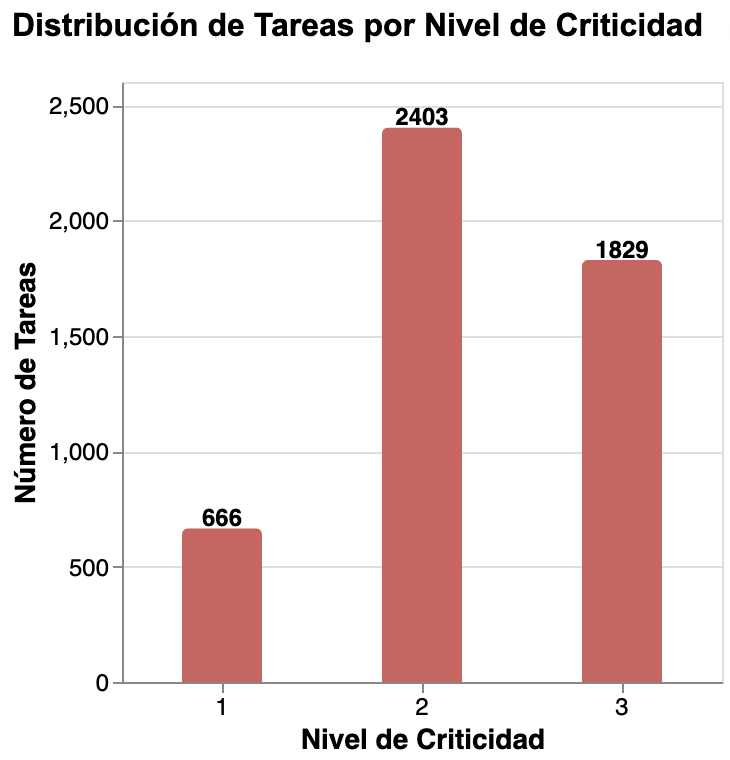
\includegraphics[width=0.5\textwidth]{imgs/barras_impacto.png}
    \caption{Distribución de tareas según su nivel de criticidad.}
    \label{fig:barras_impacto}
\end{figure}

Este conjunto de datos proporciona una base detallada y realista para el análisis y la implementación de nuestra solución, ya que combina un gran volumen de tareas con restricciones complejas y diversidad de recursos.

\subsection{Ajuste de Parámetros para la Función Objetivo}

La función objetivo del modelo combina dos componentes clave: el \textit{makespan}, representado por el parámetro \( \alpha \), y la penalización por tareas no programadas, representada por el parámetro \( \beta \). Para determinar los valores más adecuados de \( \alpha \) y \( \beta \), se llevaron a cabo múltiples experimentos utilizando diferentes combinaciones de estos parámetros. El objetivo fue evaluar cómo cada configuración afecta el equilibrio entre la minimización del \textit{makespan} y la cantidad de tareas programadas, especialmente aquellas con criticidad alta (criticidad 1).

En estos experimentos, los resultados fueron analizados en función de métricas clave, incluyendo el número total de tareas programadas, la cantidad de tareas no programadas, el makespan obtenido, el tiempo de solución requerido y la cantidad de tareas no programadas según su nivel de criticidad. Los resultados se presentan en dos cuadros: el \textbf{Cuadro~\ref{tab:alpha_beta_general}} resume las métricas generales, mientras que el \textbf{Cuadro~\ref{tab:alpha_beta_impact}} detalla la distribución de tareas no programadas según su criticidad.

\begin{table}[htbp]
    \centering
    \begin{tabular}{c>{\centering\arraybackslash}p{0.8cm} >{\centering\arraybackslash}p{0.8cm} 
                    >{\centering\arraybackslash}p{2.5cm} >{\centering\arraybackslash}p{2.5cm}
                    >{\centering\arraybackslash}p{2.5cm} >{\centering\arraybackslash}p{2.5cm}}
        \toprule
        \textbf{Conf.} & \( \alpha \) & \( \beta \) & 
        \makecell{\textbf{Tareas} \\ \textbf{Programadas}} & 
        \makecell{\textbf{Tareas no} \\ \textbf{Programadas}} & 
        \makecell{\textbf{Tiempo de} \\ \textbf{Solución (s)}} & 
        \textbf{Makespan} \\
        \midrule
        (a) & 1 & 0 & 0 & 4.898 & 3,43 & 0 \\
        (b) & 0 & 1 & 4.854 & 44 & 4,35 & 1.072 \\
        (c) & 1 & 1 & 4.658 & 240 & 8,42 & 492,75 \\
        (d) & 1 & 2 & 4.831 & 67 & 9,95 & 516,25 \\
        \bottomrule
    \end{tabular}
    \caption{Resultados generales obtenidos con diferentes configuraciones de \( \alpha \) y \( \beta \).}
    \label{tab:alpha_beta_general}
\end{table}


La configuración \( a \), donde \( \alpha = 1 \) y \( \beta = 0 \), prioriza exclusivamente la minimización del makespan. Sin embargo, este enfoque no logra programar ninguna tarea, lo que resulta inaceptable, ya que no se cumple el objetivo principal del modelo. Por otro lado, la configuración \( b \) (\( \alpha = 0 \), \( \beta = 1 \)) busca maximizar la cantidad de tareas programadas, logrando 4.854 tareas en total. Aunque esta configuración presenta un makespan elevado (1.072 horas o 44,7 días), consigue programar todas las tareas de criticidad 1, lo cual es un resultado favorable para las tareas más críticas.

La configuración \( c \) (\( \alpha = 1 \), \( \beta = 1 \)) equilibra ambos objetivos, pero a costa de una mayor cantidad de tareas no programadas (240). Si bien su \textit{makespan} es menor que el de \( b \), su penalización por dejar tareas críticas fuera del cronograma lo hace menos atractivo.

Finalmente, la configuración \( d \) (\( \alpha = 1 \), \( \beta = 2 \)) logra un balance ideal entre los objetivos de programación y makespan. Con 4.831 tareas programadas, esta configuración deja fuera solo 67 tareas (1,4\% del total), manteniendo el \textit{makespan} en un nivel razonable de 516,25 horas (21,5 días). Además, se asegura que todas las tareas de criticidad 1 son programadas, mientras que las tareas de criticidad 2 y 3 no programadas son reducidas al mínimo posible.

\begin{table}[htbp]
    \centering
    \begin{tabular}{c>{\centering\arraybackslash}p{1.5cm} >{\centering\arraybackslash}p{1.5cm} 
                    >{\centering\arraybackslash}p{1.5cm}}
        \toprule
        \textbf{Conf.} & \makecell{\textbf{Criticidad} \\ \textbf{1}} & 
        \makecell{\textbf{Criticidad} \\ \textbf{2}} & 
        \makecell{\textbf{Criticidad} \\ \textbf{3}} \\
        \midrule
        (a) & 666 & 2.403 & 1.829 \\
        (b) & 0 & 8 & 36 \\
        (c) & 21 & 59 & 160 \\
        (d) & 0 & 12 & 55 \\
        \bottomrule
    \end{tabular}
    \caption{Distribución de tareas no programadas según su criticidad.}
    \label{tab:alpha_beta_impact}
\end{table}


Se seleccionó la configuración \( d \) debido a su capacidad para satisfacer las prioridades del modelo. Aunque el tiempo de solución es el más alto entre las configuraciones evaluadas (9,95 segundos), este es un compromiso aceptable dado que garantiza un equilibrio óptimo entre la minimización del \textit{makespan} y la programación de tareas críticas. Sin embargo, este tiempo de solución podría representar un desafío operativo en escenarios más grandes. Para abordar este problema, se propone utilizar la segmentación en subconjuntos, una técnica que divide el problema en partes más manejables, reduciendo así el tiempo de cálculo necesario para resolver cada subconjunto de tareas.

\subsection{Resultados de la Segmentación en Subconjuntos}

La segmentación en subconjuntos permitió dividir el conjunto total de tareas en 14 subconjuntos más manejables, con el objetivo de reducir el tiempo de procesamiento del modelo. En el Cuadro~\ref{tab:subsets_results} se presentan los resultados obtenidos, incluyendo el número de tareas en cada subconjunto, su porcentaje relativo con respecto al total y el tiempo de solución requerido para resolver cada uno. Este análisis se llevó a cabo en un servidor virtual con las siguientes especificaciones:  

\begin{itemize}
    \item \textbf{vCPU/s:} 4 vCPUs.
    \item \textbf{RAM:} 8192 MB.
    \item \textbf{Almacenamiento:} 75 GB NVMe.
    \item \textbf{Sistema Operativo:} Ubuntu 24.10 x64.
\end{itemize}


La segmentación produjo un subconjunto principal, \( S1 \), que contiene 2.598 tareas, representando el 53\% del total. Este subconjunto, al abarcar más de la mitad de las tareas, requirió el mayor tiempo de solución (4,34 segundos). Los otros 13 subconjuntos contienen entre 68 y 674 tareas cada uno, con porcentajes significativamente menores del total. El segundo subconjunto más grande, \( S2 \), con 674 tareas (14\%), presentó un tiempo de solución de 0,65 segundos, destacando la eficiencia del enfoque modular al abordar subconjuntos de menor tamaño. Los subconjuntos más pequeños, desde \( S5 \) hasta \( S14 \), contienen menos del 5\% de las tareas totales cada uno y se resolvieron en tiempos cercanos a cero segundos.

\begin{table}[htbp]
    \centering
    \begin{tabular}{cccc}
        \toprule
        \textbf{Subconjunto} & \textbf{Número de Tareas} & \textbf{\% del Total} & \textbf{Tiempo de Solución (s)} \\
        \midrule
        \textit{S1} & 2.598 & 53\% & 4,34 \\
        \textit{S2} & 674 & 14\% & 0,65 \\
        \textit{S3} & 319 & 7\% & 0,43 \\
        \textit{S4} & 254 & 5\% & 0,12 \\
        \textit{S5} & 198 & 4\% & 0,01 \\
        \textit{S6} & 136 & 3\% & 0,01 \\
        \textit{S7} & 122 & 2\% & 0,00 \\
        \textit{S8} & 110 & 2\% & 0,01 \\
        \textit{S9} & 98 & 2\% & 0,00 \\
        \textit{S10} & 87 & 2\% & 0,00 \\
        \textit{S11} & 84 & 2\% & 0,01 \\
        \textit{S12} & 78 & 2\% & 0,00 \\
        \textit{S13} & 72 & 1\% & 0,00 \\
        \textit{S14} & 68 & 1\% & 0,00 \\
        \bottomrule
    \end{tabular}
    \caption{Resultados de la segmentación en subconjuntos.}
    \label{tab:subsets_results}
\end{table}

El procesamiento de los subconjuntos se llevó a cabo de manera paralela. Como resultado, el tiempo total de solución se igualó al máximo tiempo del \textit{solver} de todos los subconjuntos, es decir, 4,34 segundos. Este enfoque demostró la ventaja de dividir el problema en partes independientes y resolverlas simultáneamente, reduciendo considerablemente el tiempo total necesario para obtener los resultados.

\section{Conclusiones y Pasos a Seguir}


Los resultados obtenidos muestran que la solución desarrollada cumple con los objetivos propuestos al iniciar el trabajo, proporcionando una solución eficiente y satisfactoria para la programación automatizada de actividades de mantenimiento. Se logra un cronograma que cumple con las condiciones y restricciones definidas, en tiempos de procesamiento acotados y manejables.

Para nuestro conjunto de datos de 4.898 tareas, la solución logra programar el 98,6\% de las tareas, dejando solo 67 tareas no programadas. Además, se garantiza la programación de todas las tareas de criticidad 1, lo que refleja la priorización de las actividades más críticas. El \textit{makespan} obtenido es de 21,5 días, lo que indica una distribución eficiente de las tareas en el tiempo disponible.

El tiempo total de cálculo para resolver el problema completo fue de 6,12 segundos, contando el tiempo de Pre-Procesamiento, segmentación en subconjuntos, resolución de los subconjuntos y Post-Procesamiento. Consideramos este tiempo de cálculo como razonable. En la Figura \ref{fig:gantt-project} se muestra un ejemplo de un cronograma generado por la solución, en formato compatible con \textit{Microsoft Project}.


\begin{figure}[htbp]
    \centering
    \frame{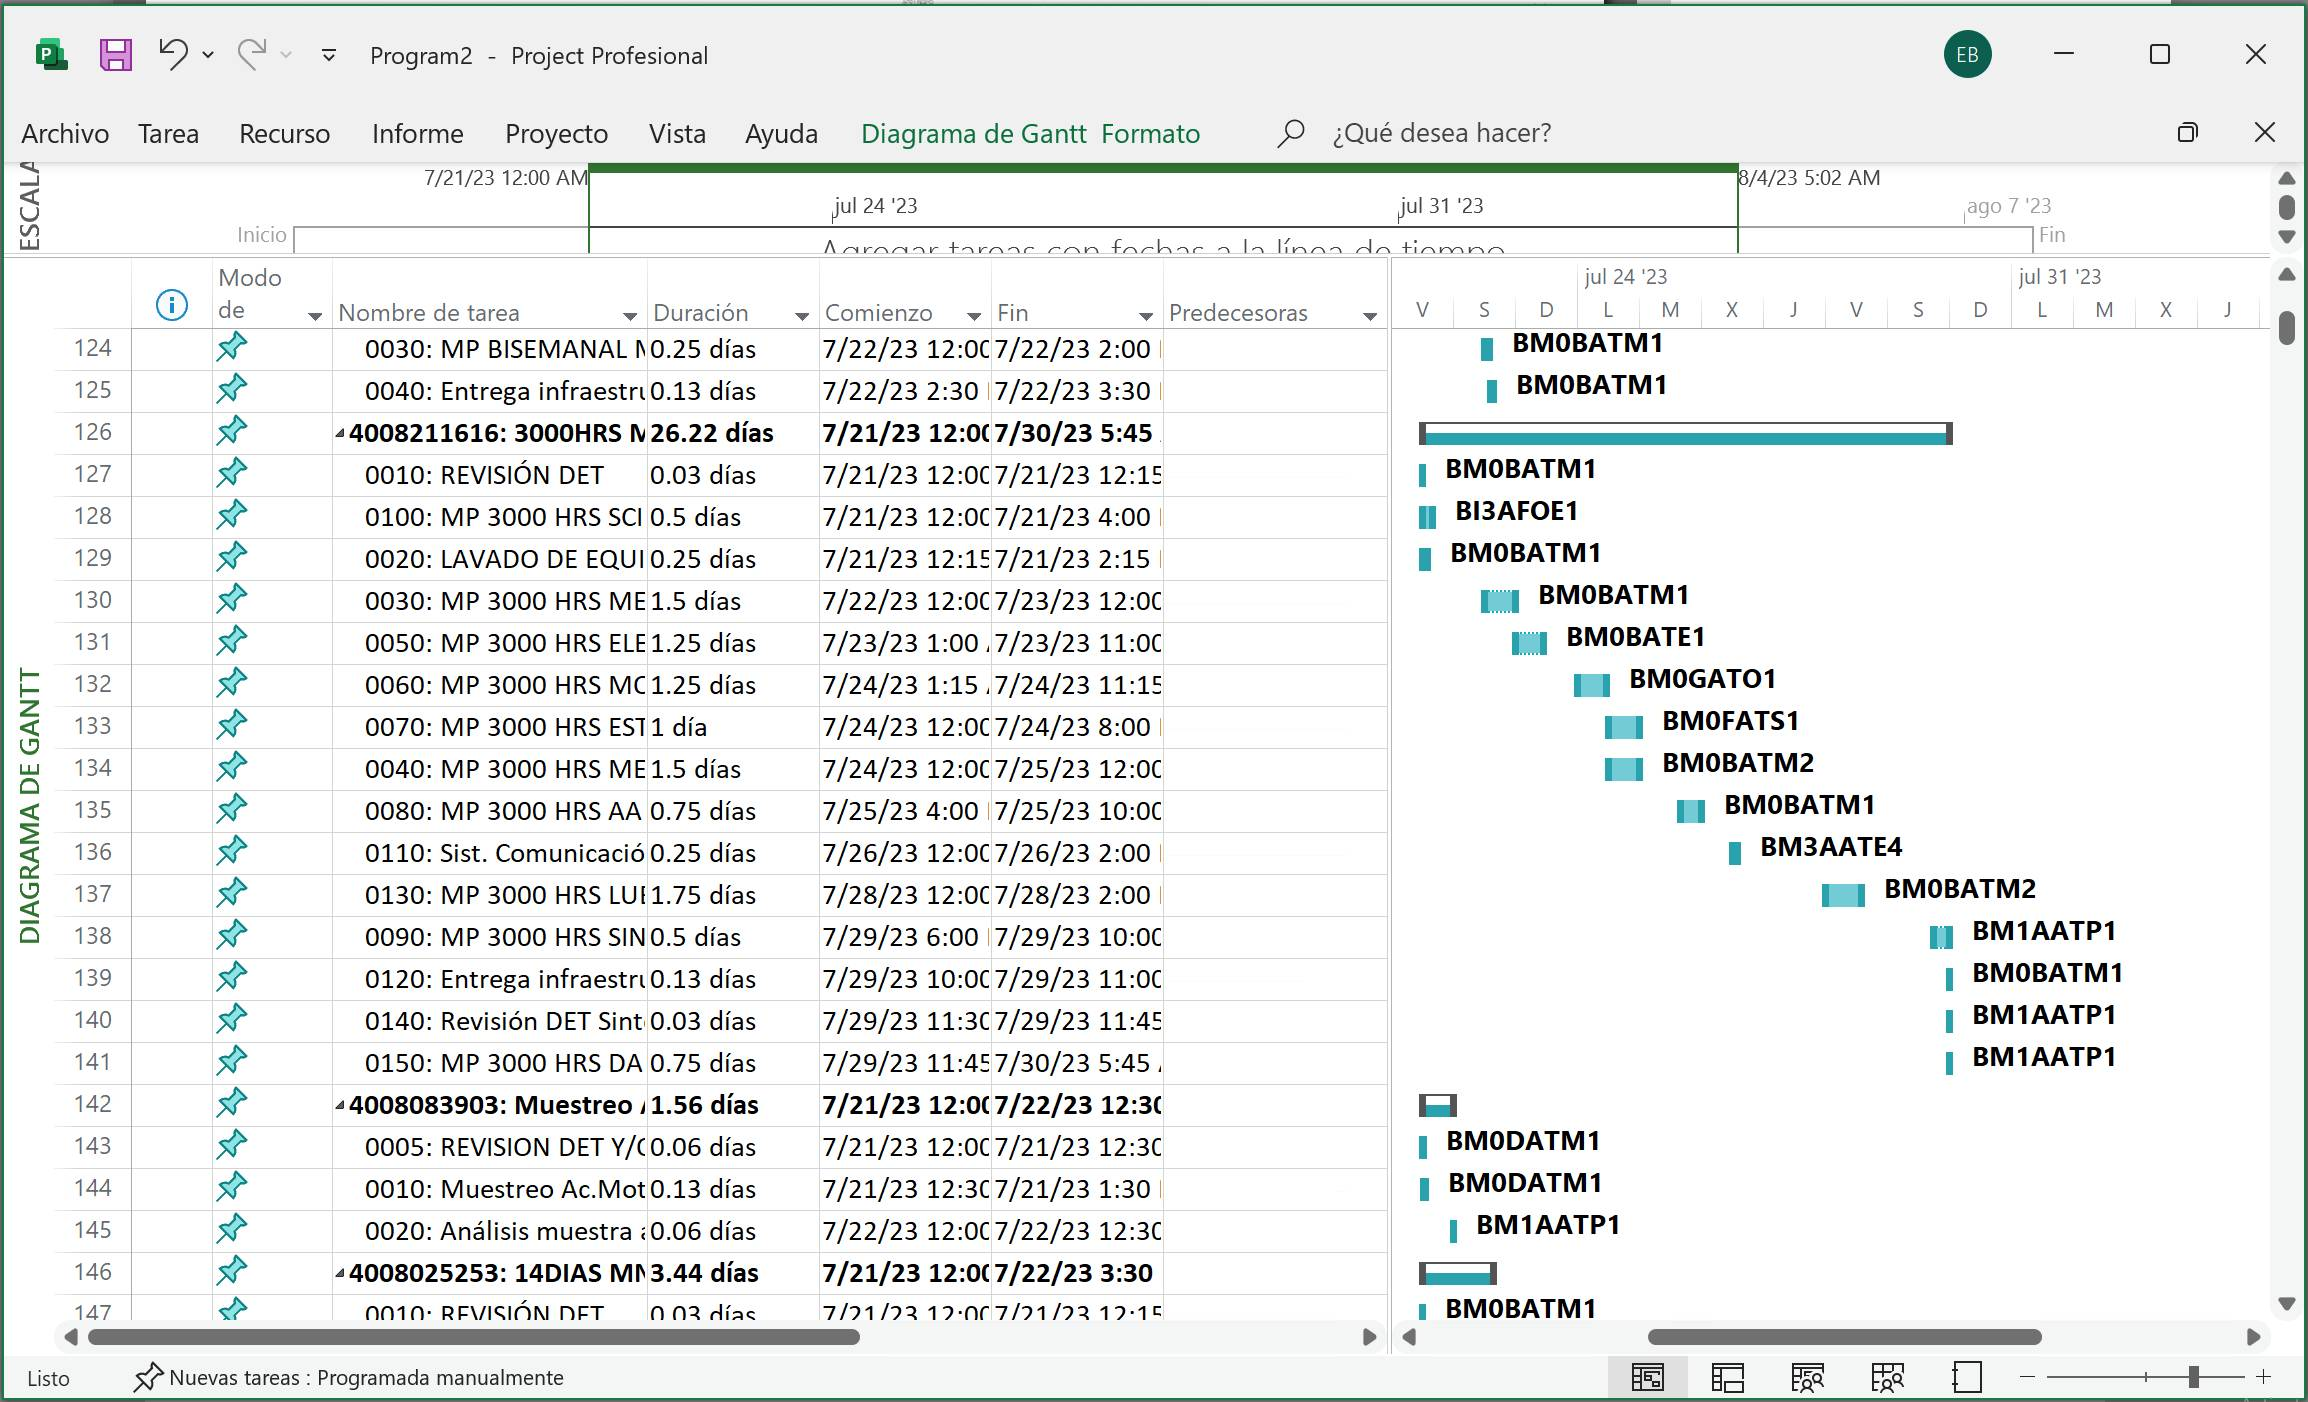
\includegraphics[scale=0.3]{imgs/gantt-project.jpg}}
    \caption{Captura de Cronograma Resultante en \textit{MS Project}}
    \label{fig:gantt-project}
  \end{figure}


\subsection{Impacto sobre Proceso de Programación}

Estimamos que la solución desarrollada puede tener un impacto significativo en la optimización del proceso de programación de actividades de mantenimiento en la empresa colaboradora. En primer lugar, permite generar un primer borrador del cronograma de forma automatizada, eliminando completamente la necesidad de realizar esta tarea manualmente. Dado que la generación del borrador inicial representa aproximadamente el 35\% del tiempo total dedicado por el equipo de programación a la creación del cronograma\footnote{Ver Anexo \ref{anexo:encuesta}}, la automatización de esta etapa por sí sola ya implica un ahorro considerable en la dedicación horaria.

Además, la solución ofrece funcionalidades para realizar ajustes finos al cronograma. Permite a los usuarios fijar una tarea en un horario específico, modificar la disponibilidad de recursos o incorporar tareas de último minuto de manera sencilla y rápida. El modelo es capaz de adaptarse rápidamente a estos cambios, recalculando un cronograma óptimo que respete las nuevas restricciones, pero sin distanciarse significativamente del cronograma inicial. Esto asegura que los ajustes sean incorporados de manera eficiente y con un mínimo de interrupciones.


Considerando que las actividades de ``Resolver conflictos de recursos'' y ``Resolver conflictos de recursos'' ocupan un 24\% y un 22\% respectivamente del tiempo total dedicado a la creación del cronograma\footnote{Ver Anexo \ref{anexo:encuesta}}, estas funcionalidades de ajuste automático podrían reducir significativamente el tiempo dedicado a estas tareas. Se estima que el tiempo dedicado a estas actividades podría reducirse a la mitad.

Por lo tanto, en términos generales \textbf{estimamos que la herramienta permite reducir en aproximadamente un 57,6\%  el tiempo total dedicado a la creación y ajuste del cronograma de tareas de mantenimiento}. Esto no solo libera al equipo de programación de una parte importante del trabajo manual, sino que también les permite enfocar su tiempo y esfuerzo en actividades estratégicas que agreguen mayor valor a las operaciones de la empresa colaboradora.

\subsection{Limitaciones y Consideraciones}

La principal limitación de nuestra solución surge de un punto identificado en la encuesta realizada al personal de programación de la empresa colaboradora, donde se destacó que el error más común derivado de una programación deficiente es la no disponibilidad de materiales y repuestos. Este problema representa un desafío crítico para garantizar la eficacia de las labores de mantenimiento. Sin embargo, en la actualidad, los datos relacionados con la disponibilidad de materiales y repuestos no están sistematizados de manera que permitan su integración con nuestra solución.

Para superar esta limitación, sería necesario implementar un paso previo enfocado en la gobernanza de datos, que incluya la elaboración de procedimientos robustos para el manejo de la información en bodega, además de programas de capacitación para los equipos responsables. También podrían ser necesarios desarrollos tecnológicos adicionales para estructurar y sistematizar estos datos de manera adecuada, permitiendo su uso dentro de nuestra solución.

Mientras estos pasos no se lleven a cabo, no podemos garantizar que nuestra herramienta reduzca los errores relacionados con la no disponibilidad de materiales y repuestos. Este aspecto requiere la colaboración y el compromiso de otras áreas de la empresa para establecer una base sólida de información confiable que pueda integrarse eficazmente al sistema de programación automatizada.

\subsection{Pasos a Seguir}

Es importante mencionar que el desarrollo del modelo y su implementación en un entorno operativo real requiere de una serie de pasos adicionales. A continuación, se detallan las recomendaciones para la implementación exitosa de la solución propuesta.

La solución se desarrolla de manera modular, estructurándose en tres componentes principales: el backend, el frontend y la integración con las plataformas de la empresa colaboradora (Ver \textbf{Figura \ref{fig:modulos-desarrollo}}). Esta división permite organizar el flujo de trabajo de forma eficiente y facilita la colaboración con el equipo técnico de la empresa, asegurando que la solución se adapte adecuadamente a sus necesidades.

\begin{figure}[htbp]
  \centering
  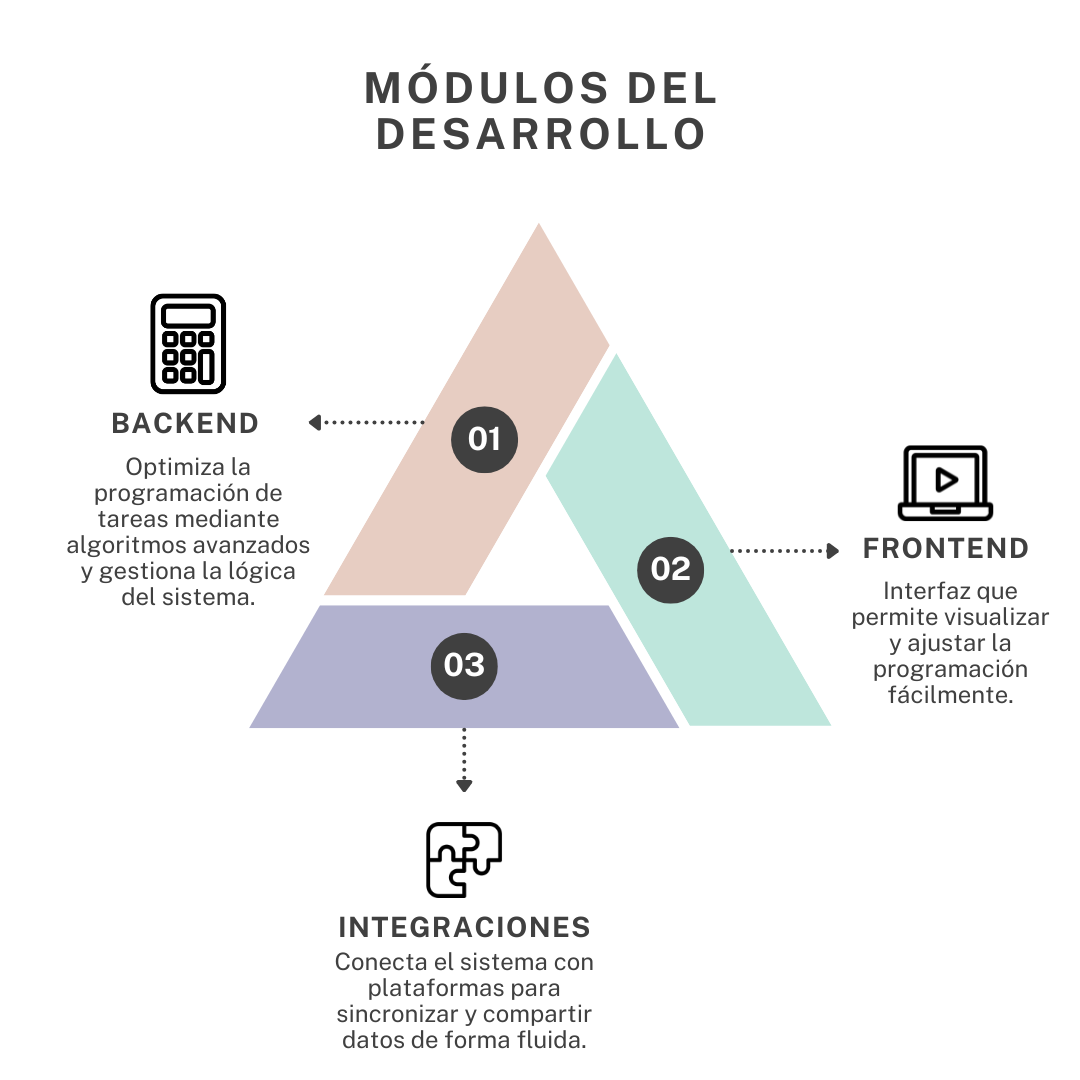
\includegraphics[scale=0.3]{imgs/ModulosDesarrollo.png}
  \caption{Propuesta de Módulos de Desarrollo de Solución}
  \label{fig:modulos-desarrollo}
\end{figure}

\subsubsection{Backend}

Para el desarrollo del backend, se sugiere utilizar frameworks como \textit{FastAPI} para exponer los endpoints REST necesarios. El motor de optimización debe implementarse mediante \textit{OR-Tools}, utilizando técnicas de \textit{CP}.

Es recomendable emplear una base de datos relacional, como \textit{PostgreSQL}, para el almacenamiento de datos relacionados con las órdenes de trabajo y las restricciones. El despliegue del backend puede realizarse utilizando contenedores \textit{Docker}, orquestados mediante un clúster de \textit{Kubernetes}. Este enfoque permite garantizar la escalabilidad, alta disponibilidad y una integración fluida con servicios en la nube. La elección del proveedor de nube (por ejemplo, \textit{AWS}, \textit{Azure}, \textit{GCP} u otros) debe basarse en las necesidades específicas de la empresa colaboradora, asegurándose de que los entornos de despliegue sean compatibles y seguros.

\subsubsection{Frontend}

El frontend debe ser diseñado como una interfaz intuitiva y eficiente, destinada a los programadores de la empresa, quienes serán los principales usuarios de la herramienta. Se recomienda que esta interfaz permita cargar datos de las órdenes de trabajo de manera sencilla, ya sea mediante la integración con un \textit{ERP} o mediante una carga masiva manual.

El desarrollo del frontend puede realizarse utilizando \textit{React.js} u otro framework moderno de JavaScript, con librerías como \textit{React-Gantt-Chart} o \textit{D3.js} para ofrecer gráficos interactivos que faciliten la visualización y edición manual de los cronogramas generados. También es aconsejable incluir funcionalidades de exportación del cronograma en formatos compatibles con \textit{MS Project} y \textit{MS Excel}, adaptándose a los flujos de trabajo ya establecidos en la empresa.

Para su despliegue, el frontend puede implementarse como una aplicación web en un entorno cloud compatible con las necesidades de la organización.

\subsubsection{Integración con Plataformas de la Empresa}

Es fundamental garantizar la integración de la solución con las plataformas existentes de la empresa, particularmente con los sistemas \textit{ERP} y otros sistemas de gestión de datos. Esta integración debe diseñarse para ser bidireccional, permitiendo tanto la importación como la exportación de información relevante de manera fluida.

Se recomienda configurar procesos automáticos para importar datos esenciales como las órdenes de trabajo, la disponibilidad de cuadrillas y los recursos necesarios desde el \textit{ERP} u otras plataformas internas. Del mismo modo, el cronograma final debe exportarse en formatos compatibles con los sistemas existentes, para su validación y distribución dentro de la organización.

Se aconseja emplear herramientas de gestión de APIs que permitan monitorear y administrar las conexiones entre los distintos módulos. Este enfoque asegura la interoperabilidad de la solución con el ecosistema tecnológico existente, adaptándose a las necesidades específicas de la empresa colaboradora.


\subsection{Reflexiones Finales}  

La solución desarrollada representa un avance significativo en la automatización de la programación de actividades de mantenimiento, con el potencial de optimizar el flujo de trabajo, reducir errores y mejorar la eficiencia operativa. La implementación de los pasos a seguir garantizará que esta solución pase de ser un prototipo a una herramienta integrada y funcional que genere un impacto tangible en las operaciones de la empresa colaboradora.


\newpage

\begin{appendix}
    \section{Resultados Encuesta sobre Programación de Actividades en el Área de Mantenimiento de la empresa colaboradora}
    \label{anexo:encuesta}

    \section*{Resumen Ejecutivo}

    Se realizó una encuesta a 19 programadores del área de mantenimiento de 6 operaciones de la empresa colaboradora, con el objetivo de identificar los principales desafíos y oportunidades de mejora en el proceso de programación. La encuesta abordó aspectos como dedicación horaria, actividades realizadas, errores comunes y problemas asociados a la coordinación.
    
    Las principales conclusiones son:
    
    \begin{itemize}
        \item \textbf{Alta dedicación horaria}: 64\% de los encuestados invierte más de la mitad de su jornada semanal en generación del cronograma de actividades.
        \item \textbf{La creación del borrador inicial} es la fase más intensiva en tiempo, superando otras actividades como resolver conflictos o validar con otras áreas.
        \item \textbf{La no disponibilidad de materiales y repuestos} durante la ejecución de las mantenciones es el error más recurrente.
        \item \textbf{Entorno altamente dinámico}: El 90\% de los encuestados enfrenta cambios de último minuto al menos una vez por semana.
        \item \textbf{Problemas de coordinación con otras áreas} y \textbf{falta de colaboración} son barreras adicionales que dificultan la programación eficiente.
    \end{itemize}
    
    Los resultados de la encuesta muestran que el proceso de programación podría beneficiarse significativamente de herramientas que automaticen partes claves del proceso. Una herramienta de automatización que permita generar el borrador inicial del cronograma, incorporar facilmente cambios de último minuto y realizar ajustes derivados de conflictos de recursos o validaciones \textbf{podría reducir en un 57,6\% la dedicación horaria del equipo de programación} en lo que respecta a la creación del cronograma de tareas. 
    
    Su éxito dependerá de su integración con las fuentes de información adecuadas, especialmente con bodega, para garantizar la disponibilidad de materiales y repuestos. Con información precisa y confiable, esta herramienta también \textbf{podría disminuir hasta en un 74\% los errores en las labores de mantenimiento derivados de una programación deficiente}.
    
    \section*{Metodología}
    
    La encuesta se aplicó a un total de 19 programadores de 6 operaciones de la empresa colaboradora, mediante una plataforma on-line, durante el mes de Diciembre de 2024. Se trató de un cuestionario breve, compuesto por 7 preguntas. La mediana del tiempo de respuesta fue de aproximadamente 5 minutos y 30 segundos. 
    
    Las preguntas estuvieron diseñadas para estimar el tiempo dedicado a la programación, la distribución de dicho tiempo entre distintas actividades, la frecuencia e impacto de errores, y las condiciones cambiantes que inciden en la planificación.
    
    A continuación se presentan los resultados y el análisis de las respuestas obtenidas.
    
    \section*{Resultados de la Encuesta}
    
    En esta sección se presentan las preguntas realizadas a los encuestados junto con un cuadro que resume los resultados obtenidos. Posteriormente, se incluye un comentario que analiza los datos presentados y destaca las principales conclusiones relacionadas con cada pregunta.
    
    \vspace{.5em}
    \subsubsection*{Pregunta 1: ¿Cuántas horas a la semana dedica el equipo de programación a generar el cronograma de tareas?}
    
    
    
    \begin{table}[htbp]
        \centering
        \begin{tabular}{lcc}
            \toprule
            \textbf{Rango de horas} & \textbf{Porcentaje} & \textbf{Cantidad} \\
            \midrule
            Menos de 10 horas & 5\% & 1 \\
            Entre 10 y 20 horas & 32\% & 6 \\
            Entre 20 y 40 horas & 53\% & 10 \\
            Más de 40 horas & 11\% & 2 \\
            \bottomrule
        \end{tabular}
        \label{tab:horas_semanales}
    \end{table}
    
    \paragraph{Comentario} Es notable que más de la mitad de los encuestados (53\%) dedica entre 20 y 40 horas semanales a la programación. Esto sugiere que la generación del cronograma de tareas consume una parte significativa de la jornada: en 64\% de los casos, más de la mitad de la semana laboral.
    
    
    \vspace{1.5em}
    \subsubsection*{Pregunta 2: ¿Qué porcentaje del tiempo total de programación está dedicado a las siguientes actividades?}
    \vspace{.5em}
    
    \begin{table}[htbp]
        \centering
        \begin{tabular}{lccc c}
            \toprule
            \textbf{Actividad} & \textbf{Promedio (\%)} & \textbf{Mínimo (\%)} & \textbf{Máximo (\%)} \\
            \midrule
            Generar el borrador inicial & 34.8 & 0 & 66\\
            Resolver conflictos de recursos & 23.8 & 10 & 70\\
            Validar con otras áreas & 19.7 & 10 & 40\\
            Realizar ajustes finales & 21.7 & 0 & 50\\
            \bottomrule
        \end{tabular}
        \label{tab:distribucion_actividades}
    \end{table}
    
    \paragraph{Comentario} Alrededor del 35\% del tiempo total de programación se concentra en la generación del borrador inicial, convirtiéndose en la actividad más demandante. Le siguen la resolución de conflictos de recursos y la realización de ajustes finales, con promedios cercanos al 24\% y 22\%, respectivamente. Cabe destacar que algunas personas reportan dedicar un 0\% de su tiempo a generar el borrador inicial o a realizar ajustes finales, lo que sugiere que estas etapas pueden ser asumidas por otras áreas o que ciertos roles se centran exclusivamente en validaciones o resolución de conflictos.
    
    \vspace{1.5em}
    \subsubsection*{Pregunta 3: ¿Cuántas personas del equipo participan activamente en la programación y qué porcentaje de su jornada diaria dedican a esta actividad?}
    
    A partir del análisis de las 19 respuestas obtenidas, se observa una gran variabilidad en el porcentaje de jornada diaria dedicado a la programación y en el número de personas involucradas. Las estadísticas resumen se presentan en el siguiente cuadro:
    
    \begin{table}[htbp]
        \centering
        \begin{tabular}{lcc}
            \toprule
            & \textbf{Promedio} & \textbf{Desviación Estándar} \\
            \midrule
            Número de personas & 2.8 & 1.5 \\
            Porcentaje de jornada diaria (\%) & 64.2 & 30.3 \\
            \bottomrule
        \end{tabular}
        \label{tab:estadisticas_resumen_jornada}
    \end{table}
    
    \paragraph{Comentario} Estos resultados reflejan una dispersión significativa: en algunos casos, un equipo reducido (2 personas) dedica el 100\% de su jornada a la programación, mientras que en otros equipos, más numerosos, el porcentaje de tiempo invertido es mucho menor.
    
    
    \vspace{1.5em}
    \subsubsection*{Pregunta 4: ¿Con qué frecuencia ocurren cambios de último minuto en las tareas o recursos disponibles?}
    
    \begin{table}[htbp]
        \centering
        \begin{tabular}{lcc}
            \toprule
            \textbf{Frecuencia} & \textbf{Porcentaje} & \textbf{Cantidad} \\
            \midrule
            Varias veces por semana & 42\% & 8 \\
            Semanalmente & 47\% & 9 \\
            Pocas veces al mes & 5\% & 1 \\
            Rara vez & 5\% & 1 \\
            \bottomrule
        \end{tabular}
        \label{tab:cambios_ultimo_minuto}
    \end{table}
    
    \paragraph{Comentario} Casi un 90\% del equipo enfrenta cambios de último minuto al menos una vez por semana. Esto evidencia un entorno altamente dinámico y la dificultad de anteponerse a los imprevistos en el proceso de programación.
    
    
    \vspace{1.5em}
    \subsubsection*{Pregunta 5: Cuál de estos errores es el más comun durante el proceso de programación?}
    
    \begin{table}[htbp]
        \centering
        \begin{tabular}{p{7cm}cc}
            \toprule
            \textbf{Tipo de error} & \textbf{Porcentaje} & \textbf{Cantidad} \\
            \midrule
            Cuadrilla no disponible & 0\% & 0 \\
            Herramientas o equipos no disponibles & 16\% & 3 \\
            Naves o talleres no disponibles & 0\% & 0 \\
            Materiales o repuestos no disponibles & 74\% & 14 \\
            Omisión de tareas críticas & 0\% & 0 \\
            El equipo sobre el cual se programó la mantención se encuentra ocupado & 11\% & 2 \\
            \bottomrule
        \end{tabular}
        \label{tab:errores_comunes}
    \end{table}
    
    \paragraph{Comentario} Lejos, el problema más recurrente identificado por los encuestados es la falta de materiales o repuestos disponibles, con un 74\% de respuestas. En segundo lugar, se encuentra la falta de herramientas o equipos disponibles; y en tercer lugar la coordinación deficiente que genera conflictos al programar mantenciones en equipos ocupados.
    
    Por otro lado, es destacable que algunos factores potencialmente problemáticos, como la falta de cuadrillas o de talleres disponibles, no representan un obstáculo en este contexto, ya que ninguno de los encuestados los señaló como fuente de errores. De manera similar, la omisión de tareas críticas tampoco parece ser un problema recurrente, lo que sugiere que estos asuntos se encuentran relativamente resueltos en el proceso actual.
    
    \vspace{1.5em}
    \subsubsection*{Pregunta 6: ¿Qué otros errores considera que podrían ocurrir durante el proceso de programación?}
    
    Las respuestas a esta pregunta abierta señalaron como errores adicionales frecuentes la falta de coordinación con otras áreas, la inclusión de actividades de último minuto, y las dificultades para coordinar a los diferentes especialistas involucrados en una tarea. También se mencionaron problemas relacionados con la falta de repuestos y la indisponibilidad de equipos auxiliares, fechas de mantenciones variables, y cambios operacionales o provenientes de otras áreas. Además, se destacó la información deficiente desde bodega en relación con los repuestos.
    
    \paragraph{Comentario} En conjunto, estas respuestas cualitativas confirman nuevamente la existencia de problemas significativos relacionados con la disponibilidad de materiales y repuestos, en gran parte vinculados a la información deficiente proporcionada por bodega. Sin embargo, también se destacan con frecuencia los problemas de coordinación con otras áreas, que reflejan desafíos relacionados con la alineación de procesos y la colaboración entre equipos.
    
    \vspace{1.5em}
    \subsubsection*{Pregunta 7: En promedio, ¿cuántos de estos errores ocurren por mes?}
    
    \begin{table}[htbp]
        \centering
        \begin{tabular}{p{7cm}cccc}
            \toprule
            \textbf{Tipo de error} & \textbf{Promedio} & \textbf{Mínimo} & \textbf{Máximo} \\
            \midrule
            Cuadrilla no disponible & 3.5 & 0 & 10 \\
            Herramientas o equipos no disponibles & 3.9 & 1 & 12 \\
            Naves o talleres no disponibles & 2.7 & 0 & 10 \\
            Omisión de tareas críticas & 2.4 & 0 & 6 \\
            El equipo sobre el cual se programó la mantención se encuentra ocupado & 3.9 & 1 & 12 \\
            Materiales o repuestos no disponibles & 6.3 & 1 & 14 \\
            \bottomrule
        \end{tabular}
        \label{tab:errores_especificos}
    \end{table}
    
    \paragraph{Comentario}La falta de materiales o repuestos disponibles vuelve a ser un factor crítico, con un promedio superior a 6 eventos por mes. Esto confirma la relevancia de contar con información fidedigna e integrada sobre la disponibilidad de recursos para mejorar la eficiencia del proceso de programación. Le siguen en frecuencia la falta de herramientas o equipos disponibles y la ocupación de los equipos programados para mantenciones, con un promedio de 3.9 eventos por mes cada uno.
    
    \section*{Análisis y Conclusiones}
    
    El análisis de los resultados de la encuesta resalta varios aspectos críticos que afectan el proceso de programación de las actividades de mantenimiento de la empresa colaboradora. Entre los hallazgos principales, destaca la alta dedicación horaria, con un 64\% de los encuestados invirtiendo más de la mitad de su jornada semanal en la generación del cronograma de tareas. La creación del borrador inicial se identifica como la etapa más demandante, representando en promedio el 35\% del tiempo total dedicado.
    
    El entorno de programación se caracteriza por ser altamente dinámico, con el 90\% de los encuestados reportando cambios de último minuto al menos semanalmente. Los errores más recurrentes están relacionados con la disponibilidad de materiales y repuestos, mencionados por el 74\% de los participantes, seguidos por la falta de herramientas y equipos auxiliares. Adicionalmente, los problemas de coordinación con otras áreas y la falta de colaboración surgen como barreras relevantes que dificultan la planificación efectiva.
    
    Los resultados de la encuesta muestran que el proceso de programación de actividades de mantenimiento \uline{podría beneficiarse significativamente de herramientas que automatizan partes clave del proceso}. En particular, una herramienta que automatice la creación del borrador inicial del cronograma y que permita incorporar de forma fluida cambios de último minuto o ajustes derivados de la resolución de conflictos de recursos y validaciones con otras áreas sería altamente efectiva. Una herramienta de este tipo, que facilite la incorporación rápida de modificaciones, \textbf{podría reducir hasta en un 57,5\% la dedicación horaria} de los equipos de programación a esta tarea, optimizando el uso de su tiempo.
    
    El éxito de esta herramienta, sin embargo, dependerá en gran medida de su integración con las fuentes de información de otras áreas de la empresa. En particular, será esencial conectarla con el área de planificación para acceder a información crítica sobre las tareas, como sus requerimientos de recursos, ventanas de tiempo (fechas de inicio más tempranas y fechas requeridas), y restricciones operativas. Además, será crucial integrarla con la información de bodega para garantizar la disponibilidad de materiales y repuestos, así como también con los datos sobre la disponibilidad de equipos. Es posible que se necesite revisar y ajustar los procedimientos de estas áreas para garantizar que la información sea precisa y confiable. Si se logra implementar una herramienta que integre estas funcionalidades y asegure la calidad de los datos, los \textbf{errores en las labores de mantenimiento derivados de una programación deficiente podrían reducirse en alrededor de un 74\%}.
    
    
\end{appendix}

\printbibliography

\end{document}
